%%%%%%%%%%%%%%%%%%%%%%%%%%%%%%%%%%%%%%%%%%%%%%%%%%%%%%%%%%%%%%%%%%%%%%
% Template for a UBC-compliant dissertation
% At the minimum, you will need to change the information found
% after the "Document meta-data"
%
%!TEX TS-program = pdflatex
%!TEX encoding = UTF-8 Unicode

%% The ubcdiss class provides several options:
%%   fogscopy
%%       set parameters to exactly how FoGS specifies
%%         * single-sided
%%         * page-numbering starts from title page
%%         * the lists of figures and tables have each entry prefixed
%%           with 'Figure' or 'Table'
%%       This can be tested by `\iffogscopy ... \else ... \fi'
%%   10pt, 11pt, 12pt
%%       set default font size
%%   oneside, twoside
%%       whether to format for single-sided or double-sided printing
%%   balanced
%%       when double-sided, ensure page content is centred
%%       rather than slightly offset (the default)
%%   singlespacing, onehalfspacing, doublespacing
%%       set default inter-line text spacing; the ubcdiss class
%%       provides \textspacing to revert to this configured spacing
%%   draft
%%       disable more intensive processing, such as including
%%       graphics, etc.
%%

% For submission to FoGS
\documentclass[fogscopy,onehalfspacing,11pt]{ubcdiss}

% For your own copies (looks nicer)
% \documentclass[balanced,twoside,11pt]{ubcdiss}

%%%%%%%%%%%%%%%%%%%%%%%%%%%%%%%%%%%%%%%%%%%%%%%%%%%%%%%%%%%%%%%%%%%%%%
%%%%%%%%%%%%%%%%%%%%%%%%%%%%%%%%%%%%%%%%%%%%%%%%%%%%%%%%%%%%%%%%%%%%%%
%%
%% FONTS:
%% 
%% The defaults below configures Times Roman for the serif font,
%% Helvetica for the sans serif font, and Courier for the
%% typewriter-style font.  Configuring fonts can be time
%% consuming; we recommend skipping to END FONTS!
%% 
%% If you're feeling brave, have lots of time, and wish to use one
%% your platform's native fonts, see the commented out bits below for
%% XeTeX/XeLaTeX.  This is not for the faint at heart. 
%% (And shouldn't you be writing? :-)
%%

%% NFSS font specification (New Font Selection Scheme)
\usepackage{times,mathptmx,courier}
\usepackage[scaled=.92]{helvet}

%% Math or theory people may want to include the handy AMS macros
%\usepackage{amssymb}
%\usepackage{amsmath}
%\usepackage{amsfonts}

%% The pifont package provides access to the elements in the dingbat font.   
%% Use \ding{##} for a particular dingbat (see p7 of psnfss2e.pdf)
%%   Useful:
%%     51,52 different forms of a checkmark
%%     54,55,56 different forms of a cross (saltyre)
%%     172-181 are 1-10 in open circle (serif)
%%     182-191 are 1-10 black circle (serif)
%%     192-201 are 1-10 in open circle (sans serif)
%%     202-211 are 1-10 in black circle (sans serif)
%% \begin{dinglist}{##}\item... or dingautolist (which auto-increments)
%% to create a bullet list with the provided character.
\usepackage{pifont}

%%%%%%%%%%%%%%%%%%%%%%%%%%%%%%%%%%%%%%%%%%%%%%%%%%%%%%%%%%%%%%%%%%%%%%
%% Configure fonts for XeTeX / XeLaTeX using the fontspec package.
%% Be sure to check out the fontspec documentation.
%\usepackage{fontspec,xltxtra,xunicode}	% required
%\defaultfontfeatures{Mapping=tex-text}	% recommended
%% Minion Pro and Myriad Pro are shipped with some versions of
%% Adobe Reader.  Adobe representatives have commented that these
%% fonts can be used outside of Adobe Reader.
%\setromanfont[Numbers=OldStyle]{Minion Pro}
%\setsansfont[Numbers=OldStyle,Scale=MatchLowercase]{Myriad Pro}
%\setmonofont[Scale=MatchLowercase]{Andale Mono}

%% Other alternatives:
%\setromanfont[Mapping=tex-text]{Adobe Caslon}
%\setsansfont[Scale=MatchLowercase]{Gill Sans}
%\setsansfont[Scale=MatchLowercase,Mapping=tex-text]{Futura}
%\setmonofont[Scale=MatchLowercase]{Andale Mono}
%\newfontfamily{\SYM}[Scale=0.9]{Zapf Dingbats}
%% END FONTS
%%%%%%%%%%%%%%%%%%%%%%%%%%%%%%%%%%%%%%%%%%%%%%%%%%%%%%%%%%%%%%%%%%%%%%
%%%%%%%%%%%%%%%%%%%%%%%%%%%%%%%%%%%%%%%%%%%%%%%%%%%%%%%%%%%%%%%%%%%%%%



%%%%%%%%%%%%%%%%%%%%%%%%%%%%%%%%%%%%%%%%%%%%%%%%%%%%%%%%%%%%%%%%%%%%%%
%%%%%%%%%%%%%%%%%%%%%%%%%%%%%%%%%%%%%%%%%%%%%%%%%%%%%%%%%%%%%%%%%%%%%%
%%
%% Recommended packages
%%
\usepackage{checkend}	% better error messages on left-open environments
\usepackage{graphicx}	% for incorporating external images

%% booktabs: provides some special commands for typesetting tables as used
%% in excellent journals.  Ignore the examples in the Lamport book!
\usepackage{booktabs}

%% listings: useful support for including source code listings, with
%% optional special keyword formatting.  The \lstset{} causes
%% the text to be typeset in a smaller sans serif font, with
%% proportional spacing.
\usepackage{listings}
\lstset{basicstyle=\sffamily\scriptsize,showstringspaces=false,fontadjust}

%% The acronym package provides support for defining acronyms, providing
%% their expansion when first used, and building glossaries.  See the
%% example in glossary.tex and the example usage throughout the example
%% document.
%% NOTE: to use \MakeTextLowercase in the \acsfont command below,
%%   we *must* use the `nohyperlinks' option -- it causes errors with
%%   hyperref otherwise.  See Section 5.2 in the ``LaTeX 2e for Class
%%   and Package Writers Guide'' (clsguide.pdf) for details.
\usepackage[printonlyused,nohyperlinks]{acronym}
%% The ubcdiss.cls loads the `textcase' package which provides commands
%% for upper-casing and lower-casing text.  The following causes
%% the acronym package to typeset acronyms in small-caps
%% as recommended by Bringhurst.
\renewcommand{\acsfont}[1]{{\scshape \MakeTextLowercase{#1}}}

%% color: add support for expressing colour models.  Grey can be used
%% to great effect to emphasize other parts of a graphic or text.
%% For an excellent set of examples, see Tufte's "Visual Display of
%% Quantitative Information" or "Envisioning Information".
\usepackage{color}
\definecolor{greytext}{gray}{0.5}

%% comment: provides a new {comment} environment: all text inside the
%% environment is ignored.
%%   \begin{comment} ignored text ... \end{comment}
\usepackage{comment}

%% The natbib package provides more sophisticated citing commands
%% such as \citeauthor{} to provide the author names of a work,
%% \citet{} to produce an author-and-reference citation,
%% \citep{} to produce a parenthetical citation.
%% We use \citeeg{} to provide examples
\usepackage[numbers,sort&compress]{natbib}
\newcommand{\citeeg}[1]{\citep[e.g.,][]{#1}}

%% The titlesec package provides commands to vary how chapter and
%% section titles are typeset.  The following uses more compact
%% spacings above and below the title.  The titleformat that follow
%% ensure chapter/section titles are set in singlespace.
\usepackage[compact]{titlesec}
\titleformat*{\section}{\singlespacing\raggedright\bfseries\Large}
\titleformat*{\subsection}{\singlespacing\raggedright\bfseries\large}
\titleformat*{\subsubsection}{\singlespacing\raggedright\bfseries}
\titleformat*{\paragraph}{\singlespacing\raggedright\itshape}

%% The caption package provides support for varying how table and
%% figure captions are typeset.
\usepackage[format=hang,indention=-1cm,labelfont={bf},margin=1em]{caption}

%% url: for typesetting URLs and smart(er) hyphenation.
%% \url{http://...} 
\usepackage{url}
\urlstyle{sf}	% typeset urls in sans-serif


%%%%%%%%%%%%%%%%%%%%%%%%%%%%%%%%%%%%%%%%%%%%%%%%%%%%%%%%%%%%%%%%%%%%%%
%%%%%%%%%%%%%%%%%%%%%%%%%%%%%%%%%%%%%%%%%%%%%%%%%%%%%%%%%%%%%%%%%%%%%%
%%
%% Possibly useful packages: you may need to explicitly install
%% these from CTAN if they aren't part of your distribution;
%% teTeX seems to ship with a smaller base than MikTeX and MacTeX.
%%
%\usepackage{pdfpages}	% insert pages from other PDF files
%\usepackage{longtable}	% provide tables spanning multiple pages
%\usepackage{chngpage}	% support changing the page widths on demand
%\usepackage{tabularx}	% an enhanced tabular environment

%% enumitem: support pausing and resuming enumerate environments.
%\usepackage{enumitem}

%% rotating: provides two environments, sidewaystable and sidewaysfigure,
%% for typesetting tables and figures in landscape mode.  
%\usepackage{rotating}

%% subfig: provides for including subfigures within a figure,
%% and includes being able to separately reference the subfigures.
%\usepackage{subfig}

%% ragged2e: provides several new new commands \Centering, \RaggedLeft,
%% \RaggedRight and \justifying and new environments Center, FlushLeft,
%% FlushRight and justify, which set ragged text and are easily
%% configurable to allow hyphenation.
%\usepackage{ragged2e}

%% The ulem package provides a \sout{} for striking out text and
%% \xout for crossing out text.  The normalem and normalbf are
%% necessary as the package messes with the emphasis and bold fonts
%% otherwise.
%\usepackage[normalem,normalbf]{ulem}    % for \sout

%%%%%%%%%%%%%%%%%%%%%%%%%%%%%%%%%%%%%%%%%%%%%%%%%%%%%%%%%%%%%%%%%%%%%%
%% HYPERREF:
%% The hyperref package provides for embedding hyperlinks into your
%% document.  By default the table of contents, references, citations,
%% and footnotes are hyperlinked.
%%
%% Hyperref provides a very handy command for doing cross-references:
%% \autoref{}.  This is similar to \ref{} and \pageref{} except that
%% it automagically puts in the *type* of reference.  For example,
%% referencing a figure's label will put the text `Figure 3.4'.
%% And the text will be hyperlinked to the appropriate place in the
%% document.
%%
%% Generally hyperref should appear after most other packages

%% The following puts hyperlinks in very faint grey boxes.
%% The `pagebackref' causes the references in the bibliography to have
%% back-references to the citing page; `backref' puts the citing section
%% number.  See further below for other examples of using hyperref.
%% 2009/12/09: now use `linktocpage' (Jacek Kisynski): FoGS now prefers
%%   that the ToC, LoF, LoT place the hyperlink on the page number,
%%   rather than the entry text.
\usepackage[bookmarks,bookmarksnumbered,%
    citebordercolor={0.8 0.8 0.8},filebordercolor={0.8 0.8 0.8},%
    linkbordercolor={0.8 0.8 0.8},pagebordercolor={0.8 0.8 0.8},%
    urlbordercolor={0.8 0.8 0.8},%
    pagebackref,linktocpage%
    ]{hyperref}
%% The following change how the the back-references text is typeset in a
%% bibliography when `backref' or `pagebackref' are used
\renewcommand\backrefpagesname{\(\rightarrow\) pages}
\renewcommand\backref{\textcolor{greytext} \backrefpagesname\ }

%% The following uses most defaults, which causes hyperlinks to be
%% surrounded by colourful boxes; the colours are only visible in
%% PDFs and don't show up when printed:
%\usepackage[bookmarks,bookmarksnumbered]{hyperref}

%% The following disables the colourful boxes around hyperlinks.
%\usepackage[bookmarks,bookmarksnumbered,pdfborder={0 0 0}]{hyperref}

%% The following disables all hyperlinking, but still enabled use of
%% \autoref{}
%\usepackage[draft]{hyperref}

%% The following commands causes chapter and section references to
%% uppercase the part name.
\renewcommand{\chapterautorefname}{Chapter}
\renewcommand{\sectionautorefname}{Section}
\renewcommand{\subsectionautorefname}{Section}
\renewcommand{\subsubsectionautorefname}{Section}


%%%%%%%%%%%%%%%%%%%%%%%%%%%%%%%%%%%%%%%%%%%%%%%%%%%%%%%%%%%%%%%%%%%%%%
%%%%%%%%%%%%%%%%%%%%%%%%%%%%%%%%%%%%%%%%%%%%%%%%%%%%%%%%%%%%%%%%%%%%%%
%%
%% Some special settings that controls how text is typeset
%%
% \raggedbottom		% pages don't have to line up nicely on the last line
% \sloppy		% be a bit more relaxed in inter-word spacing
% \clubpenalty=10000	% try harder to avoid orphans
% \widowpenalty=10000	% try harder to avoid widows
% \tolerance=1000

%% And include some of our own useful macros
% This file provides examples of some useful macros for typesetting
% dissertations.  None of the macros defined here are necessary beyond
% for the template documentation, so feel free to change, remove, and add
% your own definitions.
%
% We recommend that you define macros to separate the semantics
% of the things you write from how they are presented.  For example,
% you'll see definitions below for a macro \file{}: by using
% \file{} consistently in the text, we can change how filenames
% are typeset simply by changing the definition of \file{} in
% this file.
% 
%% The following is a directive for TeXShop to indicate the main file
%%!TEX root = diss.tex

\newcommand{\NA}{\textsc{n/a}}	% for "not applicable"
\newcommand{\eg}{e.g.,\ }	% proper form of examples (\eg a, b, c)
\newcommand{\ie}{i.e.,\ }	% proper form for that is (\ie a, b, c)
\newcommand{\etal}{\emph{et al}}

% Some useful macros for typesetting terms.
\newcommand{\file}[1]{\texttt{#1}}
\newcommand{\class}[1]{\texttt{#1}}
\newcommand{\latexpackage}[1]{\href{http://www.ctan.org/macros/latex/contrib/#1}{\texttt{#1}}}
\newcommand{\latexmiscpackage}[1]{\href{http://www.ctan.org/macros/latex/contrib/misc/#1.sty}{\texttt{#1}}}
\newcommand{\env}[1]{\texttt{#1}}
\newcommand{\BibTeX}{Bib\TeX}

% Define a command \doi{} to typeset a digital object identifier (DOI).
% Note: if the following definition raise an error, then you likely
% have an ancient version of url.sty.  Either find a more recent version
% (3.1 or later work fine) and simply copy it into this directory,  or
% comment out the following two lines and uncomment the third.
\DeclareUrlCommand\DOI{}
\newcommand{\doi}[1]{\href{http://dx.doi.org/#1}{\DOI{doi:#1}}}
%\newcommand{\doi}[1]{\href{http://dx.doi.org/#1}{doi:#1}}

% Useful macro to reference an online document with a hyperlink
% as well with the URL explicitly listed in a footnote
% #1: the URL
% #2: the anchoring text
\newcommand{\webref}[2]{\href{#1}{#2}\footnote{\url{#1}}}

% epigraph is a nice environment for typesetting quotations
\makeatletter
\newenvironment{epigraph}{%
	\begin{flushright}
	\begin{minipage}{\columnwidth-0.75in}
	\begin{flushright}
	\@ifundefined{singlespacing}{}{\singlespacing}%
    }{
	\end{flushright}
	\end{minipage}
	\end{flushright}}
\makeatother

% \FIXME{} is a useful macro for noting things needing to be changed.
% The following definition will also output a warning to the console
\newcommand{\FIXME}[1]{\typeout{**FIXME** #1}\textbf{[FIXME: #1]}}

% END


%%%%%%%%%%%%%%%%%%%%%%%%%%%%%%%%%%%%%%%%%%%%%%%%%%%%%%%%%%%%%%%%%%%%%%
%%%%%%%%%%%%%%%%%%%%%%%%%%%%%%%%%%%%%%%%%%%%%%%%%%%%%%%%%%%%%%%%%%%%%%
%%
%% Document meta-data: be sure to also change the \hypersetup information
%%

\title{Optimal Planning with Approximate Model-Based Reinforcement Learning}
%\subtitle{If you want a subtitle}

\author{Hai Feng Kao}
\previousdegree{M.Sc., National Taiwan University, 2006}
\previousdegree{B.Sc., National Taiwan University, 2004}

% What is this dissertation for?
\degreetitle{Master of Science}

\institution{The University Of British Columbia}
\campus{Vancouver}

\faculty{The Faculty of Graduate Studies}
\department{Computer Science}
\submissionmonth{April}
\submissionyear{2011}

%% hyperref package provides support for embedding meta-data in .PDF
%% files
\hypersetup{
  pdftitle={Master Thesis(DRAFT: \today)},
  pdfauthor={Hai Feng Kao},
  pdfkeywords={Reinforcement Learning}
}

%%%%%%%%%%%%%%%%%%%%%%%%%%%%%%%%%%%%%%%%%%%%%%%%%%%%%%%%%%%%%%%%%%%%%%
%%%%%%%%%%%%%%%%%%%%%%%%%%%%%%%%%%%%%%%%%%%%%%%%%%%%%%%%%%%%%%%%%%%%%%
%% 
%% The document content
%%

%% LaTeX's \includeonly commands causes any uses of \include{} to only
%% include files that are in the list.  This is helpful to produce
%% subsets of your thesis (e.g., for committee members who want to see
%% the dissertation chapter by chapter).  It also saves time by 
%% avoiding reprocessing the entire file.
%\includeonly{intro,conclusions}
%\includeonly{discussion}

\begin{document}

%%%%%%%%%%%%%%%%%%%%%%%%%%%%%%%%%%%%%%%%%%%%%%%%%%
%% From Thesis Components: Tradtional Thesis
%% <http://www.grad.ubc.ca/students/thesis/index.asp?menu=003,000,000,000>

% Preliminary Pages (numbered in lower case Roman numerals)
%    1. Title page (mandatory)
\maketitle

%    2. Abstract (mandatory - maximum 350 words)
%% The following is a directive for TeXShop to indicate the main file
%%!TEX root = diss.tex

%Introduction
%RL->MDP, Q, SARSA, SMDP, 
%MAXQ (include the algorithm), hierarchical optimal vs recursive optimal, HORDQ, Relational,  Model-based RL (cite Peter Stone's Model based approach and a brief intro of it, include the algorithm)
%the problem of HO
%Optimal planning, model the differences
%scale to large problems
%The power of model-based RL and relational approach--> use a maze to illustrate this(model the difference)
%Linear SARSA
%Super Mario

%Motivation:
%1. scale to large problem with small number of samples

%chpater 2: 
%1. MaxQ

%chapter 3:
%1. The power of model based approach--> one wall sample and one pincecess can solve the whole maze problem
   %1.1. show the effectiveness
   %1.2. scaling up--> a noval biased model-based approach (show that it is the only way)
   %1.3. the necessity of biased approach
   %1.4. the choice between planning variable and not
   %1.5. wrong decision variable causes disater (decision)

%chapter 4:
%1. the three optimality ()
%2. Combined with hierarchical optimal RL
%3. why we need leaf cover
%4. the convergence for online approach
%5. the offiline one
%6. Respect the hierarchy

%chpater 5 scaling it up
%1. Better generalization: relational rl
%1.1. the power of model the difference
%2. Reduce training time: transfer learning
%3. case study: Super Mario

%chapter 6 future work
%1. make it hierarchical optimal (add only put down to get passenger subtask in taxi domain)
%2. A general way to combine any approximated model-based approach and can still achieve optimality
\chapter{Abstract}

Model-based reinforcement learning methods make efficient use of samples by
building a model of the environment and planning with it. Compared to
model-free methods, they usually take fewer samples to converge to the optimal
policy. Despite that efficiency, model-based methods may not learn the optimal
policy due to structural modeling assumptions. In this thesis, we show that by
combining model-based methods with hierarchically optimal recursive Q-learning (HORDQ)
under a hierarchical reinforcement learning framework, the proposed approach
learns the optimal policy even when the assumptions of the model are not
satisfied.
%we propose a simple approach that assumes most of the variables are static
%during the planning process and focuses on modeling the few dynamic variables.

% Embed version information inline -- you should remove this from your
% dissertation
\vfill
\begin{center}
\begin{sf}
\fbox{Revision: ubcdiss.cls r27
}
\end{sf}
\end{center}

\cleardoublepage

%    3. Table of contents (mandatory - list all items in the preliminary pages
%    starting with the abstract, followed by chapter headings and
%    subheadings, bibliographies and appendices)
\tableofcontents
\cleardoublepage	% required by tocloft package

%    4. List of tables (mandatory if thesis has tables)
\listoftables
\cleardoublepage	% required by tocloft package

%    5. List of figures (mandatory if thesis has figures)
\listoffigures
\cleardoublepage	% required by tocloft package

%    6. List of illustrations (mandatory if thesis has illustrations)
%    7. Lists of symbols, abbreviations or other (optional)

%    8. Glossary (optional)
%%% The following is a directive for TeXShop to indicate the main file
%%!TEX root = diss.tex

\chapter{Glossary}

This glossary uses the handy \latexpackage{acroynym} package to automatically
maintain the glossary.  It uses the package's \texttt{printonlyused}
option to include only those acronyms explicitly referenced in the
\LaTeX\ source.

% use \acrodef to define an acronym, but no listing
\acrodef{UI}{user interface}
\acrodef{UBC}{University of British Columbia}

% The acronym environment will typeset only those acronyms that were
% *actually used* in the course of the document
\begin{acronym}[ANOVA]
\acro{ANOVA}[ANOVA]{Analysis of Variance\acroextra{, a set of
  statistical techniques to identify sources of variability between groups}}
\acro{API}{application programming interface}
\acro{CTAN}{\acroextra{The }Common \TeX\ Archive Network}
\acro{DOI}{Document Object Identifier\acroextra{ (see
    \url{http://doi.org})}}
\acro{FoGS}[FoGS]{The Faculty of Graduate Studies}
\acro{PDF}{Portable Document Format}
\acro{RCS}[RCS]{Revision control system\acroextra{, a software
    tool for tracking changes to a set of files}}
\acro{TLX}[TLX]{Task Load Index\acroextra{, an instrument for gauging
  the subjective mental workload experienced by a human in performing
  a task}}
\acro{UML}{Unified Modelling Language\acroextra{, a visual language
    for modelling the structure of software artefacts}}
\acro{URL}{Unique Resource Locator\acroextra{, used to describe a
    means for obtaining some resource on the world wide web}}
\acro{W3C}[W3C]{\acroextra{the }World Wide Web Consortium\acroextra{,
    the standards body for web technologies}}
\acro{XML}{Extensible Markup Language}
\end{acronym}

% You can also use \newacro{}{} to only define acronyms
% but without explictly creating a glossary
% 
% \newacro{ANOVA}[ANOVA]{Analysis of Variance\acroextra{, a set of
%   statistical techniques to identify sources of variability between groups.}}
% \newacro{API}[API]{application programming interface}
% \newacro{GOMS}[GOMS]{Goals, Operators, Methods, and Selection\acroextra{,
%   a framework for usability analysis.}}
% \newacro{TLX}[TLX]{Task Load Index\acroextra{, an instrument for gauging
%   the subjective mental workload experienced by a human in performing
%   a task.}}
% \newacro{UI}[UI]{user interface}
% \newacro{UML}[UML]{Unified Modelling Language}
% \newacro{W3C}[W3C]{World Wide Web Consortium}
% \newacro{XML}[XML]{Extensible Markup Language}
	% always input, since other macros may rely on it

\textspacing		% begin one-half or double spacing

%    9. Preface (optional)
%   10. Acknowledgements (optional)
%% The following is a directive for TeXShop to indicate the main file
%%!TEX root = diss.tex

\chapter{Acknowledgments}

I am very fortunate to have the opportunity to study and do research in
University of British Columbia. I am most grateful to my supervisor, Alan Mackworth.
When I proposed the idea of developing a generic game AI for video games, he
accepted and allowed me to work on a problem which I am really passionate about.
Besides, I would like to thank David Buchman, John Chia and Bruno Norberto da Silva
for sharing their knowledge and expertise in reinforcement learning.
%Without his encouragement and kindness, I would have gave up this idea long before.
I would also like to thank Tzu-Kuo Huang for sharing
the new research works done at CMU. One of the works actually inspired
the idea of this thesis.
A special thank goes to Prof. Poole, who gave me many precious ideas to make this
thesis better.
And most importantly, I would like to thank my parents, who support
me whenever I need it. Without them, it is impossible to finish this work.
%Thank those people who helped you. 

%Don't forget your parents or loved ones.

%You may wish to acknowledge your funding sources.

%I have been very fortunate to have an enjoyable and fruitful learning experience here in
%University of Alberta, and for this I am most grateful to my supervisor, Michael Bowling.
%He has provided me with the opportunity to work on a research topic that I am truly
%passionate about, given me enough academic freedom to experiment and learn on my own,
%and yet he has always been there to guide me when I was lost and confused.
%I am very thankful to my fellow graduate students who have generously and patiently
%shared their knowledge and expertise and have been instrumental for the completion of this
%thesis. In particular, I would like to thank Marc Lanctot and Chris Rayner for sharing their
%knowledge and getting me started with the Atari 2600 hardware and the emulation tools,
%Mohammad Shaei for sharing his insights on the concepts behind the UCT algorithm,
%and Michael Johanson for oering his expertise on running batch simulations on computer
%clusters. Our late night discussions with Amir-Massoud Farahmand have been some of the
%best learning experiences I have had through the last two years. I am very grateful to him,
%who has been both an inspiring colleague and a good friend.
%I am indebted to the team behind Stella, the Atari 2600 emulator, for releasing their
%work as open-source and allowing me to build my toolset on top of their code. I would
%also like to thank Richard Sutton and the RLAI group for releasing the source code of their
%Tile-Coding and Sarsa() implementations. I hope that releasing my own code base as
%open-source will be similarly benecial to other researchers and hobbyists.

%I would like to thank my supervisor, Michiel van de Panne, for his continuous
%support, guidance, and his willingness to let me explore the research tangents
%that made my time here so enjoyable. Michiel's joyful excitement about the
%eld is infectious, and I will cherish the times we spent reverse-engineering
%the human and animal motor system. The insights I gained through our
%discussions about academia have been particularly helpful and shaped me
%as a researcher.
%I am also thankful to Nando de Freitas for contributing ideas to this project,
%and for helping me with this thesis. I had the opportunity to closely interact
%with Nando on many projects and endeavors over the last two years, and
%his support, excitement, and can-do attitude have been very helpful and
%inspiring.
%I would also like to extend my thanks to David Lowe, Bob Woodham, and
%Kevin Murphy, all of whom I've come to know and admire over the last two
%years. I also had the pleasure of working with Steve Wolfman and Kimberly
%Voll as a TA on several occasions, and I am thankful to have witnessed their
%inspiring dedication to teaching.
%My thanks go to my bullpen mates and lab mates Paul Vanetti, John Chia,
%Byron Knoll, Stelian Coros, Philippe Beaudoin, Ben Jones, and many others
%who I don't have enough space to name for contributing to a pleasant, fun
%working atmosphere and oering healthy distractions from work.
%I wish to thank my sister for her unconditional support, and my parents,
%who sacriced to bring us to Canada and made it possible for me to pursue
%my dreams.
%Last but not least, I wish to thank Shelly, for giving me something to look
%forward to every day.

%I thank my advisor Alan Mackworth for being extremely supportive, friendly and
%amazingly open to very different research ideas. It is incredible how you manage to
%keep me on track without restricting the paths I choose to follow. Your generosity
%and helpfulness are a great lesson that I hope I can replicate one day with my own
%students. You are an idol.
%I’m grateful for all my LCI colleagues, for the stimulating environment and
%support. I learned a lot from many of you. A special note goes to Prof Giuseppe
%Carenini who helped me with my PhD application and 
%All my family in Brazil, for all the emails, phone calls, thoughts. Thanks for
%all your patience, care, support. And I’m trying hard to find the time to go back
%and see you all again.
%ma femme. Nao sei se devo repetir os votos ou se
%referencio minhas teses de graduacao e mestrado. Em todo caso, Helena fica aqui
%registrada como a motivacao e inspiracao deste e de todo meu trabalho.



%   11. Dedication (optional)

% Body of Thesis (not all sections may apply)
\mainmatter

\acresetall	% reset all acronyms used so far

%    1. Introduction
%% The following is a directive for TeXShop to indicate the main file
%%!TEX root = diss.tex

\chapter{Introduction}
\label{ch:intro}

\section{Problem Statement}
The objective of this project is to build a software which can play a wide range 
of video games. To achieve this goal, the software shall not possess any game-specific 
information. Besides, the software shall be able to play the games in a non-intrusive approach.
That is, the software shall be able to extract the necessary information 
from the screenshot of the games and control the games from standard input devices such as keyboard.
Since most of video games use graphical display as the primary interface, this requirement allows
the software to be applied to different video games.

\section{Why video games?}
Over the past decade, substantial research has been conducted to teach computer play classic strategy games such
as Deep Thought\cite{DeepBlue}, TD-Gammon\cite{Gammon}, and GO\cite{Go}.
On the other hand, little research has been made\cite{FPS}\cite{Mario} to extend the effort to other genres of video games.
The genres of video games include not only classic strategy games, but also action, first-person shooter, role-player, adventure, simulation, etc.
Video games introduce a new challenge to the AI community.

The challenge includes:
\begin{itemize}{}

\item A generic algorithm which can adapt to different types of games:
Following the paradigm of \cite{GGP} and \cite{Yavar}, the objective is not to design a good AI for
a specific game. Instead, the objective is to design a good and generic AI to play different games successfully.

\item Large but highly structured states:
For a 256 color video game with resolution $640 \times 480$, it has $256^(640 \times 480)$ states.
The number states are too big to be tractable. However, a video game often consists of small number of objects.
If we can figure out a way to represent the relationship of these objects, the number of states
can be reduced.

\item Dynamic number of agents:
Unlike classic strategy games, the number of agents in video games is highly dynamic.
The number of agents may increase over time and decrease if killed.
It is a challenge which doesn't exist in classic strategy games.
\end{itemize}

Video games can be viewed as a abstract representation of the real world. Often can we find the 
correspondence between such an artificial world to a real-world problem\cite{KeepAway}.
Focusing on Video games allows us to attack a real-world problem without tackling unnecessary details, while maintaining sufficient 
level of abstraction. In addition, video games are well-understood and customizable environments. 
It allows us to test an AI algorithm and justify if the result is correct\cite{Yavar}.

Another possible application is the AI of video games.
Nowadays, the AI engineers usually need to craft the behavior of AI by hand. 
The process are time-consuming and the hard-coded behavior would produce unrealistic AI behavior.
If we can design a generic agent and let it act reactively with the environment, it can produce 
more various and unpredictable behaviors.

\section{Why applying computer vision to video games?}

The reason behind is the reality that most of the video games do not have source codes which are publicly available.
If a researcher needs to test his algorithm on Super Mario Bros., all he can do is to apply it on Infinite Mario Bros.,
which is an open source clone of original Super Mario Bros. He cannot test his algorithm on Mario Bros. 1 or 2, which are available
on binary format. If a researcher does not have source codes, he cannot extract the game states like the location
of Koopa Troopas which are mandatory for any AI algorithm to work. 

Using computer vision techniques to extract the information from the game screen is a way to solve this problem.
Because most of the video games uses graphics as the primary interface to interact with the player, it contains
the necessary information for the player to play. The use of computer vision allows us to test the algorithm
non-intrusively, without the effort to hack the game engine or reimplement the game.

Besides, the vision allows a more generic way for a computer to play a video game. It creates 
new applications which cannot be done by intrusive approaches.

\begin{itemize}{}
\item Non-intrusive and generic AI:
Have you ever played a good game with poor AI? Can you change it with a better one?
Without the source codes of the game or the engine support, the answer is usually "No".
Nevertheless, if we could design a software which can learn to play any video game, 
the answer can be changed to "Yes". The non-intrusive and generic agents can be 
applied to any video games with/without the support from the game company.

\item Modding: 
Game modding becomes popular in recent years \cite{Modding}. 
Modding allows users to customize the video games to suite their personal tastes.
The modding usually includes the introduce new content, modification of original one, or remove the unsatisfactory elements.
The process can be done by the support of game development kit released by the game company.
It can also be done without the support from the game company. However, the modders need to hack the game engine,
decode the data format and implement their own development kit. 
The process can be time-consuming and tedious.
If we could automate the process by having a software which can 
traverse the game and extract the in-game elements for us, it could save a lot of time.

\end{itemize}

%\chapter{Related Work}
%\label{ch:Related}
\section{Related Work}

There are several works which address how to design a good AI for certain type of video games.
McPartland et al. proposed a approach to allow bots in First-Person Shooter (FPS)
games to learn how to navigate the maze and handle combat \cite{FPS}. M. Smith et al. proposed a coordination 
framework to allow the bots to adapt to different strategy by reinforcement learning \cite{FPS_TEAM}. 
Michael et al. applied a Monte Carlo planning approach for Real-Time Strategy (RTS) gmaes to 
the Rush-the-Flag game \cite{RTS}. Ponsen et al. proposed hierarchical relational learning to learn how to play
the Battle of Survival game \cite{HRRL}. For arcade-style games, \cite{Mario} uses a RL agent to learn
how to play Infinite Mario Bro. Driessens et al. proposed a relational RL to learn how to play the Digger
game. In \cite{OO}, a object-oriented representation is proposed to play pitfall.

Previous works rely on the intrusive approach to provide the states of games for the agents to play.
The agents need to know the information such as the number of objects, the types of objects,
or the health level of players to play the games. The intrusive approach makes it difficult to generalize
to a large number of video games. And the game-specific representation prevents these approaches
to be applied to arbitrary video games.

With the objective to play general video games, our work is most related to 
General Game Playing\cite{GGP} (GGP) and Playing Atari 2600 \cite{Yavar}. 
The objective of GGP is to develop a software agent which can play unspecific games if the rules
are given. Our work follows the same objective. However, due to the complexity of video games, 
it is not clear that how to precisely describe the rules of video games.

Y. Naddaf\cite{Yavar} proposed A.L.E. (Atari 2600 Learning Environment) as the platform to test AI algorithms.
A.L.E. supports fast emulation and generic interface. Fast emulation allows the emulator to run 
games without rendering or sound generation. It can increase the speed in the learning phase.
The generic interface provides AI agents the screenshot and scores in games. It allows us
to build the agents in a game independent way.

Our work is built on A.L.E. However, our work differs from \cite{Yavar} in the following perspective:

\begin{itemize}{}
\item Our work features object-based representation. We argue that objects are the fundamental elements
in video games. The representation allows the agent to develop appropriate policy against specific 
objects. And it also enables the possibility to reuse the knowledge in different stages.
\end{itemize}

\chapter{Reinforcement Learning}
\label{ch:RL}
The objective of reinforcement learning algorithm is to build an learning agent. The learning agent will take
actions based on the current state. In the beginning, the agent does not know anything about 
the environment, therefore the agent has to choose the first action randomly. After the environment
receives the action, it will provide a reward to the agent as a feedback. The reward can be either
positive or negative.

The agent adjusts the value function to maximize the expected reward in the future.
The value function represent the expected reward when the agent takes certain action in the current
state, and it is used to estimate the "quality" of an action. The initial value of value function is 
usually 0, but it is possible to set it to some high enough value to encourage exploration.
It is important to evaluate the value function 
correctly. If some actions with low expected reward are estimated as high, it degrades the
performance of agent.

The agent can select an action which leads to the highest value of value function. However, 
this strategy does not allow the agent to explore the states which are not visited before.
A better approach is to use $\epsilon$-greedy method. The method allows the agent to abandon the
best action and choose
a random action with a very small probability $\epsilon$. The higher the probability, the more
likely that the agent would explore the new actions. However, if the exploration probability 
is too high, it will increase the time to converge.

After the agent takes an action, the environment will provide a reward and a state to the
agent. The agent then decides an new action for the new state. After several iterations
, the agent will learn a correspondence between the action and state. The correspondence is called 
"policy". 

\section{Temporal Difference}
\label{sec:TD}
There are 3 types of reinforcement learning algorithms -- dynamic programming(DP), Monte Carlo 
methods, and temporal-difference (TD). Dynamic programming can compute the optimal policy, but it 
requires a precise model of the environment. In most of the cases, the environment
is too complex to be modeled precisely, and it is not easy to get the complete information about
the environment. On the other hand, it is usually possible to use Monte Carlo method to sample the environment to
get the partial information. 
Like Monte Carlo method, TD uses sampling, therefore it does not require the 
complete model of the environment. TD method is a bootstrapping method, similar to the dynamic 
programming approach, it updates the new value function based on the previous one.

The equation to compute the value function in TD:
\begin{displaymath}
   V(S_t) \leftarrow V(S_t) + \alpha [r_{t+1} + \gamma V(S_{t+1}) - V(S_t)],
\end{displaymath}

where $V(s_t)$ is the value function of the state $s_t$. $V(s_t)$ is the expected reward when
the agent reaches the state $s_t$. $r_{t+1}$ is the reward given to the agent when it chooses
the action at state $s_t$.

\section{SARSA}
\label{sec:SARSA}
SARSA is a on-policy TD approach. On-policy indicates that it learns from the current policy.
Different from other TD approaches, SARSA updates the Q value of the current state-action from the next state-action.
The Q value is updated by:
\begin{displaymath}
    Q(s_t, a_t) \leftarrow Q(s_t, a_t) + \alpha [r_{t+1} + \gamma Q(s_{t+1}, a_{t+1})-Q(s_t, a_t)],
\end{displaymath}
where $Q(s, a)$ is the value function for state-pair, and it is the expected reward when the agent takes
the action $a$ at the state $s$. $\alpha$ is step-wise, which controls the learning rate. 
$\gamma$ is the discount factor.


\begin{center}
\begin{tabular}{@{}lp{6cm}@{}}
\hline
Algorithm: SARSA\\
\hline
Initialize $Q(s, a)$ arbitrarily\\
Repeat (for each episode)\\
\ \ \ \ \ \ Initialize $s$\\
\ \ \ \ \ \ Choose $a$ based on $s$ using policy derived from $Q$ (e.g., $\epsilon$-greedy method)\\
\ \ \ \ \ \ Repeat (for each step of episode):\\
\ \ \ \ \ \ \ \ \ \ \ \ Take action $a$, obtain reward $r$ and next state $s'$ from the environment\\
\ \ \ \ \ \ \ \ \ \ \ \ Choose $a'$ based on $s'$ using policy derived from $Q$ (e.g., $\epsilon$-greedy method)\\
\ \ \ \ \ \ \ \ \ \ \ \ $Q(s, a) \leftarrow Q(s, a) + \alpha [r + \gamma Q(s', a')-Q(s, a)]$\\
\ \ \ \ \ \ \ \ \ \ \ \ $s \leftarrow s'$\\
\ \ \ \ \ \ \ \ \ \ \ \ $a \leftarrow a'$\\
\ \ \ \ \ \ Until $s$ is terminal\\
\hline  
\end{tabular}
\end{center}

\section{Q-Learning}
\label{sec:Q-Learning}
    Q-Learning is an off-policy TD approach. Compared to SARSA, Q-Learning updates
the Q value by the highest value of the next possible state-action, rather than the 
next state-action executed by the agent.  
The Q value is updated by:
\begin{displaymath}
   Q(s_t, a_t) \leftarrow Q(s_t, a_t) + \alpha [r_{t+1}+\gamma \max_a Q(s_{t+1},a)-Q(s_t,a_t)],
\end{displaymath}

where $\max_a Q(s_{t+1},a)$ is the highest value of the next possible state-action. 


\begin{center}
\begin{tabular}{@{}lp{6cm}@{}}
\hline
Algorithm: Q-Learning\\
\hline
Initialize $Q(s, a)$ arbitrarily\\
Repeat (for each episode)\\
\ \ \ \ \ \ Initialize $s$\\
\ \ \ \ \ \ Repeat (for each step of episode):\\
\ \ \ \ \ \ \ \ \ \ \ \ Choose $a$ based on $s$ using policy derived from $Q$ (e.g., $\epsilon$-greedy method)\\
\ \ \ \ \ \ \ \ \ \ \ \ Take action $a$, obtain reward $r$ and next state $s'$ from the environment\\
\ \ \ \ \ \ \ \ \ \ \ \ $Q(s, a) \leftarrow Q(s, a) + \alpha [r + \gamma max_{a'} Q(s', a')-Q(s, a)]$\\
\ \ \ \ \ \ \ \ \ \ \ \ $s \leftarrow s'$\\
\ \ \ \ \ \ Until $s$ is terminal\\
\hline  
\end{tabular}
\end{center}

\section{minmax Q-Learning}
\label{sec:minmax}

    In two player zero-sum game, it's reasonable to take the action of the opponent into consideration.
In minmax Q-learning, the Q value is a function of state, the action of player, and the action of opponent.
The Q value is updated by:
\begin{displaymath}
    Q(s_t, a_t, o_t) \leftarrow Q(s_t, a_t, o_t) + \alpha [r_{t+1}+\gamma\max_a min_o Q(s_{t+1}, a, o)-Q(s_t, a_t, o_t)],
\end{displaymath}

\begin{center}
\begin{tabular}{@{}lp{6cm}@{}}
\hline
Algorithm: minmax Q-learning\\
\hline
\ \ \ Initialize: $Q(s, a, o) \leftarrow 1, V(s) \leftarrow 1$
\ \ \ Repeat (for each episode)\\
\ \ \ \ \ \ Initialize $s$\\
\ \ \ \ \ \ Repeat (for each step of episode):\\
\ \ \ \ \ \ \ \ \ \ \ \ Choose $a$ based on $s$ using policy derived from $Q$ (e.g., $\epsilon$-greedy method)\\
\ \ \ \ \ \ \ \ \ \ \ \ Take action $a$, obtain opponent action $o$, reward $r$ and next state $s'$ from the environment\\
\ \ \ \ \ \ \ \ \ \ \ \ $Q(s, a, o) \leftarrow Q(s, a, o) + \alpha [r + \gamma max_{a'} min_{o'} Q(s', a', o')-Q(s, a, o)]$\\
\ \ \ \ \ \ \ \ \ \ \ \ $s \leftarrow s'$\\
\hline  
\end{tabular}
\end{center}


\chapter{Relational Learning}

Dynamic number of objects
No fixed representation
Dependency with samples. (intrinsic to reinforcement learning, since consective states has similar
Q-value, there are not independent all)

Video games involves objects: things like monsters, treasures, or princess.
But the most current machine learning algorithms requires the world to be represented 
by a vector of attributes. The vector representation has several drawbacks when applied to objects.


The vector representation is ordered. However, it's not clear how to assign a fixed for the objects.

The length of vector representation is fixed. However, the number of objects might vary.

The relationship between objects are lost in the vector representation. 

Motivation
Consider a typical questionanswering task on the
web 	BernersLee et al������  Fensel et al������ 
������
which might involve accessing and integrating semi
structured information from the web to answer a com
plex query������ eg������ nd a graduate school on the west
coast that has aordable housing������ multiple faculty and
funded research in Articial Intelligence Even if the
query is posed in a formal query language������ answer
ing it requires several skills such as query planning������
optimization������ information extraction������ and information
integration in a relational language Or consider what
is involved in learning to cook a meal While certainly
not an exhaustive list������ one needs to reason about peo
ples tastes and preferences������ ones own knowledge of
recipes and skills������ availability of ingredients������ their lo
cations������ and procedures to access them������ the capacities
of utensils and cooking ranges������ and the eects of dif
ferent proportions of ingredients������ of cooking temper
atures������ and of dierent kinds of cooking processes on
the taste and quality of the nal product
It is easy to pose both of these problems as reinforce
ment learning problems In both tasks������ we might pe
nalize the system for the time spent and other costs������
and reward it for the quality of the nal product
What is problematic������ however������ is that the structure
of the web and the reasoning involved in the cooking
task are most naturally represented using relational
representations This poses several challenges to the
success of RL in these domains
Function Approximation������ The valuefunction ap
proximation typically used in RL������ eg������ neural net
works or regression trees������ does not generalize well
when applied to relational domains This is partly
because these representations are illsuited to the
task of representing relational knowledge When
they are successful������ they require a careful choice of
propositional features or basis functions which are
handcrafted specically to a particular task at
hand Designing functionapproximation schemes
that exploit relational structure when present is a
critical challenge
Generalization across Objects������ RL methods that
do not explicitly represent objects and relation
ships between them are fundamentally limited in
their ability to transfer learning about one object
to similar related objects Critical challenges here
are identifying classes of objects that are to be
considered similar������ across which such general
ization is justied������ and identifying and represent
ing knowledge suitable for transfer
Transfer across Tasks������ RL programs are usually
tested on a single task and do not exhibit transfer
of knowledge across tasks Each task in a given
domain������ eg������ each query in information retrieval������
may look quite dierent when formulated propo
sitionally������ and thus may require separate training
to learn to answer it Relational representations
facilitate formulating broad collections of related
tasks as a single domain������ yielding natural gener
alization between these related tasks
Runtime Planning and Reasoning������ In most re
inforcement learning work������ there is no deliberate
planning and reasoning at runtime It is tac
itly assumed that either all planning occurs of
ine or the system relies completely on explo
ration and learning to construct good plans������ re
ducing the runtime execution to reactive behav
ior However������ complex dynamic domains require
both deliberation and reactivity������ as is demon
strated by successful gameplaying programs It
appears that the approximate nature of the value
function demands a more rened search at the run
time to compensate for its errors Reasoning may
also be important in constructing new features for
an improved valuefunction approximation
Prior Knowledge������ RL deemphasizes the role of
prior knowledge in learning and reasoning������ thus
relying on trial and error learning which can be
very ine
cient and often does not scale to more
complex tasks such as the above
Relational reinforcement learning 	RRL
 seeks to ad
dress all the above problems by generalizing RL to re
lationally represented states and actions In fact������ both
reinforcement learning and relational learning have a
long history The study of reinforcement learning be
gan with Samuels pioneering  work on checkers
	Samuel������ 
 Work on relational learning started
with Winstons work on blocks world learning 	Win
ston������ 
 In recent times������ relational learning is stud
ied under dierent names������ including inductive logic
programming������ relational data mining and probabilis
tic relational modeling Reinforcement learning is also
studied under multiple guises of which neurodynamic
programming and decision theoretic planning are the
most recognizable

%\section{Object-Oriented Relational Reinforcement Learning}
\section{Relational Markov Decision Processes}

Following the definition in \cite{RelationalMDP}, we define 
a relational MDP as follows:

Definition: Relational Markov decision process is formalized as a tuple $<C, S, O, D, A, T, R>$, where
\begin{itemize}{}
\item $C$ is a set of object classes $C={C_1, \dots, C_c}$. Each
class is associated with a set of state variables $S[C]={C.S_1, \dots, C.S_k}
    \item 
\end{itemize}
the system dynamics and rewards
at the level of a template for a task domain. Given a particular
environment within that domain, it defines a specific MDP
instantiated for that environment. The domain is specified by a schema,
which specifies a set of object classes $C = fC1; : : : ;Ccg. Each class
C is also associated with a set of state variables S[C] =
fC:S1; : : : ;C:Skg, which describe the state of an object in
that class. Each state variable C:S has a domain of possible
values Dom[C:S]. We define SC to be the set of possible
states for an object in C, i.e., the possible assignments to the
state variables of C.
For example, our Freecraft domain might
have classes such as Peasant, Footman, Gold;
the class Peasant may have a state variable
Task whose domain is Dom[Peasant:Task] =
fWaiting, Mining, Harvesting, Buildingg, and a state
variable Health whose domain has three values. In this
case, SPeasant would have 4  3 = 12 values, one for each
combination of values for Task and Health.
The schema also specifies a set of links L[C] =
fL1; : : : ;Llg for each class representing links between objects
in the domain. Each link C:L has a range [C:L] = C0.
For example, Peasant objects might be linked to Barrack
objects — [Peasant:BuildTarget] = Barrack, and to the
global Gold and Wood resource objects. In a more complex
situation, a link may relate C to many instances of a
class C0, which we denote by [C:L] = fC0g, for example,
[Enemy:My Footmen] = fFootmang indicates that an instance
of the enemy class may be related to many footman instances.
A particular instance of the schema is defined via a
world !, specifying the set of objects of each class; we use
O[!][C] to denote the objects in class C, and O[!] to denote
the total set of objects in !. The world ! also specifies
the links between objects, which we take to be fixed
throughout time. Thus, for each link C:L, and for each
o 2 O[!][C], ! specifies a set of objects o0 2 [C:L], denoted
o:L. For example, in a world containing 2 peasants,
we would have O[!][Peasant] = fPeasant1;Peasant2g;
if Peasant1 is building a barracks, we would have that
Peasant1:BuildTarget = Barrack1.
The dynamics and rewards of an RMDP are also defined
at the schema level. For each class, the schema
specifies an action C:A, which can take on one of several
values Dom[C:A]. For example, Dom[Peasant:A] =
fWait, Mine, Harvest, Buildg. Each class C is also associated
with a transition model PC, which specifies the probability
distribution over the next state of an object o in class
C, given the current state of o, the action taken on o, and the
states and actions of all of the objects linked to o:
PC(S0
C j SC;C:A;SC:L1 ;C:L1:A; : : : ;SC:Ll ;C:Ll:A): (1)
For example, the status of a barrack, Barrack:Status0,
depends on its status in the previous time step, on
the task performed by any peasant that could build it
(Barrack:BuiltBy:Task), on the amount of wood and gold, etc.
The transition model is conditioned on the state of C:Li,
which is, in general, an entire set of objects (e.g., the set of
peasants linked to a barrack). Thus we must now provide
a compact specification of the transition model that can depend
on the state of an unbounded number of variables. We
can deal with this issue using the idea of aggregation [10].
In Freecraft, our model uses the count aggregator ], where
the probability that Barrack:Status transitions from Unbuilt to
Built depends on ][Barrack:BuiltBy:Task = Built], the number
of peasants in Barrack:BuiltBy whose Task is Build.
Finally, we also define rewards at the class level. We assume
for simplicity that rewards are associated only with the
states of individual objects; adding more global dependencies
is possible, but complicates planning significantly. We define
a reward function RC(SC;C:A), which represents the contribution
to the reward of any object in C. For example, we
may have a reward function associated with the Enemy class,
which specifies a reward of 10 if the state of an enemy object
is Dead: REnemy(Enemy:State = Dead) = 10. We assume
that the reward for each object is bounded by Rmax.
Given a world, the RMDP uniquely defines a ground factored
MDP !, whose transition model is specified (as usual)
as a dynamic Bayesian network (DBN) [3]. The random variables
in this factored MDP are the state variables of the individual
objects o:S, for each o 2 O[!][C] and for each
S 2 S[C]. Thus, the state s of the system at a given point in
time is a vector defining the states of the individual objects in
the world. For any subset of variablesX in the model, we define
s[X] to be the part of the instantiation s that corresponds
to the variables X. The ground DBN for the transition dynamics
specifies the dependence of the variables at time t+1
on the variables at time t. The parents of a variable o:S are
the state variables of the objects o0 that are linked to o. In our
example with the two peasants, we might have the random
variables Peasant1:Task, Peasant2:Task, Barrack1:Status,
etc. The parents of the time t + 1 variable Barrack1:Status0
are the time t variables Barrack1:Status0, Peasant1:Task,
Peasant2:Task, Gold1:Amount andWood1:Amount.
The transition model is the same for all instances in the
same class, as in (1). Thus, all of the o:Status variables for

Health H’

Count
   	 
Health H’
AFootman

 
F1.Health
F1.A
F1.H’
E1.Health E1.H’
F2.Health
F2.A
F2.H’
E2.Health E2.H’

������



 	 
 
 	 
 

Time   
(a) (b)
Figure 2: Freecraft tactical domain: (a) Schema; (b) Resulting factored
MDP for a world with 2 footmen and 2 enemies.
barrack objects o share the same conditional probability distribution.
Note, however, that each specific barrack depends
on the particular peasants linked to it. Thus, the actual parents
in the DBN of the status variables for two different barrack
objects can be different.
The reward function is simply the sum of the reward functions
for the individual objects:
R(s; a) = X
C2C
X
o2O[!][C]
R(s[So]; a[o:A]):
Thus, for reward function for the Enemy class described
above, our overall reward function in a given state will be
10 times the number of dead enemies in that state.
It remains to specify the actions in the ground MDP. The
RMDP specifies a set of possible actions for every object in
the world. In a setting where only a single action can be taken
at any time step, the agent must choose both an object to
act on, and which action to perform on that object. Here,
the set of actions in the ground MDP is simply the union
[o2!Dom[o:A]. In a setting where multiple actions can be
performed in parallel (say, in a multiagent setting), it might
be possible to perform an action on every object in the domain
at every step. Here, the set of actions in the ground MDP is a
vector specifying an action for every object: o2!Dom[o:A].
Intermediate cases, allowing degrees of parallelism, are also
possible. For simplicity of presentation, we focus on the multiagent
case, such as Freecraft, where, an action is an assignment
to the action of every unit.
Example 2.1 (Freecraft tactical








































\endinput
Any text after an \endinput is ignored.
You could put scraps here or things in progress.

Objective: Allow computer to play video games
Objective2: perfect modeling
abundance of old games
home robot entertaunnent(kinetics) join the family
Approach:
Input: Screen and Reward function
1. Video Analysis 
2. Control the game by RL algorithms--RL algorithms must be able to be applied to different games successfully
3. Modeling dynamics(the agent needs to explore the game to get enough information)

Comparison to previous work:
1. Nonintrusive gaming(compared to NIPS 2008)
2. Modeling the game
Chanllenge:
1. Real-Time Video Anaylysis
2. A generic RL algorithm which works on different games
Unlike previous work on RL, the objective is not to design a good AI for a specific game to against
human player, the objective is to design a good and generic AI for play different games successfully
But it is not required to be perfect or optimal. AI in video games cannot be perfect, otherwise it 
would be not possible for a human player to beat the game. The opponent is suboptimal in nature.
3. Little prior knowledge on the games. Unlike keep away, it's not possible to design heiracial action
for (Pong). It must be able to play the game from primitive actions or construct the complex actions by itself.
Volleyball
Example: 
  Fireball vs Soccer ball
  In one game, it's necesart to intercept the soccer ball.
  In another game, it's lethal to touch any ball.
4. Huge game states(640X480X30X(256) per seconds), highly redudunet
5. Little training time (the game has 30fps), cant increase that
6. Dynamic number of agents(avoid ball)(different from soccer)(the number of player is dynamics (unlike game theory))

Motivation for reinforcement learning

Articial Intelligence algorithms that can play classic or video games have been studied ex-
tensively. Research in classic games has resulted in Deep Thought for chess [Campbell et al., 2002],
Chinook for checkers [Schaeer et al., 2005], TD-Gammon for backgammon [Tesauro, 1994],
and Polaris for poker [Bowling et al., 2009]. For AI researchers who work on solving vari-
ous games, there is a recurring question that needs to be addressed: why dedicate limited
resources to solving games instead of tackling the real-world problems in which the eld of
Articial Intelligence can contribute to the daily quality of human lives? In other words,
why spend resources on solving chess, if what we need is self-driving cars with near zero
collision rates? Why play checkers, if what we want is an intelligent maid robot that can
cook, vacuum, and wash the dishes?
The motivation for developing AI agents that can play games is threefold. First, games
oer controlled, well-understood, and easily abstracted environments, with well-dened mea-
sures of success and failure. These properties make games suitable platforms for developing
and testing AI algorithms. The methods developed and the knowledge gained from work-
ing in these controlled environments can later be applied to the real-world problems which
are generally messier and harder to measure performances, but still require the same AI
sophistication.
Additionally, games are excellent platforms for showcasing the capabilities of the latest
AI techniques to the public. In 1997, when Deep Blue defeated Garry Kasparov, a great
wave of excitement was generated among regular, non-academic people about Articial
Intelligence. This is because people understand chess, and respect the complexity involved
in playing it well. Back in 1997, the AI community was not able to develop collision-free
autonomous cars or achieve many other longer-term goals of the eld. Showcasing an agent
that mastered chess helped the public understand what the AI community was capable of
at the time.
Finally, with the recent growth of commercial video games into a multibillion-dollar
industry, there is now even more motivation for studying agents that can learn to act intelli-
gently in games [Lucas, 2009, Laird and Lent, 2000]. Non-repetitive, adaptive, interesting,
and in summary intelligent behavior oers a competitive edge for commercial games. As
the game graphics peak at image-like quality, and as the game consoles oer more and more
computational power that can be spent on complex learning algorithms, the importance of
3


Application:
1. desktop (sort the data row??)
2. gaming ( a alternative of in game AI) can act as opponent or friends (human and computer cooperation)( with 2 different computers)
3. game modeling ( convert to another platform)
2. simulatioin env forj robot
4. agent in online gaming (need to go to toilet)
5. General in game AI
6. General in computer sceice (viki, robot soccer simulated)

high level editing
4. game synthesys (chane the protagonist in game, add monsters)

Problem Statement
The objective of this project is to build a software which can play a wide range 
of video games. To achieve this goal, the software shall not possess any game-specific 
information. Besides, the software shall be able to play the games in a non-intrusive approach.
That is, the software shall be able to extract the necessary information 
from the screenshot of the games and control the games from standard input devices such as keyboard.
Since most of video games use graphic display as the primary interface, this requirement allows
the software to be applied to different video games.

Why video games?
Go beyond Chess and robot soccer:
Over the past decade, substantial research has been conducted to teach computer play classic strategy games such
as Deep Thought for chess [Campbell et al., 2002],
Chinook for checkers [Schaeer et al., 2005], TD-Gammon for backgammon [Tesauro, 1994],
go (Silver, Sutton, and Muller 2007).
and Polaris for poker [Bowling et al., 2009].
On the other hand, little research has been made [cite here] to extend the effort to other genres of video games.
The genres of video games include not only classic strategy games, but also action, first-person shooter, role-player, adventure, simulation, etc\ldots
These games introduce the new challendge to AI community
Complex, can have really large, continuous state and
action spaces.

Can we go beyond the classic ones to investigate the more diversifying video games? 

But why do we need to study suce a topic?
Nowadys, it's quite normal for game company to 
Video games can be viewed as a abstract representation of the real world. Often can we find the 
correspondence between such an ariticial world to a real-world problem<robot soccer, viki>.
Video games allow us to attack a real-world problem without tackling uncessary details, while maintaing enough 
level of abstraction.
Video games are well-understood, custimizable environments. They allow us to work test an AI algorithm
and justify if the result is correct. <alberta, Namir>

Another application is the game industry.
Nowadys, the AI engineers usually need to craft the behavior of the AI by hand. 
The process are time-comsuing and it will produce unrealistic charactor behavior.
If we can design 

Educational


Why vision on video games?

The reason behind is based on the reality that most of the video games do not have source codes publicly available.
If a researcher needs to test his RL alogrithm on Super Mario Bros., all he can do is to apply it on (infinity mario),
since it's the only Mario which goes open source. He cannot test his alrogithm on Mario 1 or 2, which are availbel
on binary. If a researher does not have a source code, he cannot extract the game state like the locaiton
of scoobma which are mandatory for any AI alogrithm. 

Using computer vision techniques to extract the information from the game screen is a way to solve this problem,
since most of the video games uses graphics as the primary interface to interact with the player, it contains
the necessary information for the player to play. The use of computer vision allows us to test the algorithm
non-intrusively, without the effort to hack the game engine or reimplement the game.

Besides, the vision allows a more generic way for a computer to play a video game. It creates 
new applications which cannot be done by intrusive approaches.

Nontrusive and generic AI:
Have you ever experience a good game with poor AI.

--------------High level modeling---------------------
Modding: 
Game modding becomes popular in recent years [modding], 
Modding allows users to customize the video games to suite their personal tastes.
The modding usually includes the introduce new content, modification of oringinal ones, remove the unsatisfactory elements.
The process is usually can be done by the support of game developement kit released by the game company.
It can also be done without the support from the game company. The players need to hacking the game engine,
to decode the data format and develope their own developlment kit. 
Eductional part: --> put the education effort to the game without engine support
It enables the possibility of Nonintrusive modding.
Reuse the AI module in other games. Reuse the content from other games

One engine rules all
In previous, video games are built from scratch. A game company first decides the types of the game,
then then developed the game engine and the content of the game. Later, people starts to figure out 
that the game engine and the content of the game can be separated. The content of the game mostly consist of
artistic materials, dialogs and simple scripte, while the game engines handle the most programming part.
To the game engine, the content is nothing but a set of data. It's more efficient to reuse the same enging
to create multiple games. The reconigction creates the game company which specialized in content, while other
focused on the content. I 
The game companies usually .
Is it possible to use one engine to run all video games?
It is a distinct dream, and cannot be done by policital force.
The modeling of video games also allows us to convert abitrary game into
some unified represention such UML. 
With the universial representation,
it creates the possibility to use one game engine, which serve as the interpret of the content, to run all video games.

It is a dream
The modeling of video games also create the possibility to use 
Platform indepent description of a video game:
There are abunadnt of old games which can 
One simulator for all games
mobile platform: iphone, gphone
web appl: play it on line flash

The modeling of the video games allows us to extract the graphics, the dynamics
and the AI in video games. It enables the possibility to reconstruct the game in 
a high level way. 
--------------High level modeling---------------------


allows the users to modify the 

There has been a recent increase in the number of game environments or engines
that allow users to customize their gaming experiences by building and
expanding game behavior. This article describes the use of modifying, or
modding, existing games as a means to learn computer science, mathematics,
physics, and aesthetic principles. We describe two exploratory case studies of
game modding in classroom settings to illustrate skills learned by students as
a result of modding existing games. We also discuss the benefits of learning
computer sciences skills


Entertainment and Educational Robot:
In the future, 
The robots are not only for chores, it will become a part of the family.
It can listen, and speak with people. 
It won't be a machine which can only execute the instruction from people.
It will give feedback to the poeple. Tell poeple the solution.
It will have be emotionally connected with people.
Teach the young generation how to use computers. 
A future that human and robot can work together and play together.
The possbility shall not be limited to physical games, but also video games.
How can a computer learns how to use another computer.

There will be emotional connection with the robots and people. 

It can play with child,
teach people how to use computer, or even play video games. 
production or domestic services





Computer vision 
1. no source code
Modding
Remodoling
Nonintrusive AI (in different computer)
Gaming robot(Teach people use computer family member, play with people, home robot not chores)
2. have source code, but hard to modify
A general way to manupulate program
3. 



Articial Intelligence algorithms that can play classic or video games have been studied ex-
tensively. Research in classic games has resulted in  For AI researchers who work on solving vari-
ous games, there is a recurring question that needs to be addressed: why dedicate limited
resources to solving games instead of tackling the real-world problems in which the eld of
Articial Intelligence can contribute to the daily quality of human lives? In other words,
why spend resources on solving chess, if what we need is self-driving cars with near zero
collision rates? Why play checkers, if what we want is an intelligent maid robot that can
cook, vacuum, and wash the dishes?
The motivation for developing AI agents that can play games is threefold. First, games
oer controlled, well-understood, and easily abstracted environments, with well-dened mea-
sures of success and failure. These properties make games suitable platforms for developing
and testing AI algorithms. The methods developed and the knowledge gained from work-
ing in these controlled environments can later be applied to the real-world problems which
are generally messier and harder to measure performances, but still require the same AI
sophistication.
Finally, with the recent growth of commercial video games into a multibillion-dollar
industry, there is now even more motivation for studying agents that can learn to act intelli-
gently in games [Lucas, 2009, Laird and Lent, 2000]. Non-repetitive, adaptive, interesting,
and in summary intelligent behavior oers a competitive edge for commercial games. As
the game graphics peak at image-like quality, and as the game consoles oer more and more
computational power that can be spent on complex learning algorithms, the importance of
3
Over the past decade substantial research has been
performed on reinforcement learning (RL) for the robotics
and multi-agent systems (MAS) fields. In addition, many
researchers have successfully used RL to teach a computer
how to play classic strategy games such as backgammon
(Tesauro 1995) and go (Silver, Sutton, and Muller 2007).
However, there has been little research in the application of
RL to modern computer games. First person shooter (FPS)
games have common features to the fields of robotics and
MAS, such as agents equipped to sense and act in their
environment, and complex continuous movement spaces.
Therefore, investigating the affects of RL in an FPS
environment is an applicable and interesting area to
research.




Beyond Soccer and chess. A new oppourtunituy.

Input of the program:
User cases:
1. Q-Learning
2. SARSA
3. MinMax Q
3. different parameter
4. different game (Pong, Robot Soccer, and Other)
5. different look ahead level of MinMaxQ in different games
6. Cite Sutton work
7. Cite Kevin work
8. Performance comparison of heuristic search vs RL
9. Make MinMaxQ work

Restriction of previous RL:
1. The incapability to generalize (think of an unvisited state)
2. Small number of states
3. fixed represention?

Why RL doesn't work:
dimension
example:
A MDP example with random object for each episode
(sol: Using pairwise Q function to model the Q value between agent and the object, the Q value is centered at the object and we sum it up to get the final Q function for the player)

Future:
A robot can understand how to use computer program in HCI approach


RBM:
action recognition and RL is the same: the diff is that the label of RL is an agent's action
1. heiracial can handle both space and time heiracy, and form the composition actions from the raw data
(solve 66 frames problem)
2. Can use the RBM result to reconstruct the game (how?) 
3. How to deal with dummy agent(action indepent of the env) with real agent(action depends on the env)
4. How to reuse the policy against a certain type of agent to a new unknown agent?
5. How to put the action of an agent into the hierachy? Using supervise human player video is possible, how about unsupervised?
If I can make it work, then the jitter problem of an user agent can be solved(action performed in a reduced dim, no small scale action problem anymore)
How to form a hierachical action policy?
Can use a supervised soccer video to train an agent? therefore the agent can learn the complex action automatically. (keep away soccer)
use a prior to penalize the jitter of an agent's action



6. order the objects from near to far and include the objects action in previous frame



7. the relationship between SOM
8. use different level to quantize the location of the ball and the opponent(use the past 100 frame to predict the future)
9. use different level to model the action of the players(intuition: the dim of the optimal policy is very small)
10. Question: how to create hierachical policy?
11. Iuition: the RL should be both scale and time invariant (if the movement is 0.001 pixel per frame, it should also work)
12. Model the strategy of opponent into macro action, and use them to defeat the opponent. (most video games has built-in AI, can just learn from that, 慕容復?)
If no opponent, then we have to rely on human.
13. treat action as missing data
14. intuition: the ball movement and the enemy movement are deterministic in most of the games. Therefore the dimension is pretty low.
15. For high frame rate game (like 120 FPS), it's necessary to model the opponent behavior to get the intrinsic action space
otherwise, the random walk is too slow. Or consider the Wolf 3D maze(big maze and small movement). It's too hard to rely on random walk to find the exit.
Each action replies on each expert. The switch action is equal to switch expert. (Hinton's RBM RL)
The qeustion is: when to switch the action? How to handle the big action space problem(can it be small?)
16. Cooperation ML(viki.eecs.harvald.edu)
17. curvature turning is a way to detect the boundary of an macro action (to model the opponent action)(curvature on location(x y) or action(up down left right)?)
It is better to apply it to Andrej's work on virtual avatar walking(human joint movement at walking in 1 dim)
18. create Q value from the actions in the same cluster (same scenario), combine different Q function to build a hierachy(locally trained)
19. Pong->tennis(more strategy, counter attack may fail)
20. Learning from opponent
21. MinMax SMDP Q learning
22. Copy paste programming for video games
23. Genetic algorithm from ada-boosting (you can choose different subset of training data to create different combination 
of actions)
24. collision detection as a prior information is still a way to go (pair-wise relationship modeling)
25. David: Model the transition matrix and immediate reward and use MDP instead.
26. Use convoltition to generate pairwise relationship to multiple objects--> A Q function which centered at a block which contains 
3 objects. (spatial hierachy)
27. Fictitous gameplay with convolution. If I have pairwise model, I can simulated the game by put the player in a 
small block which contains 3 or five objects and simulated the real Q function using pairwise model.
28. The answer of taxi driver problem shall be HMM. It is nothing but first order temporal model. (each temporal
state has different task and therefore has different Q function(a function of time))
29. Convert 2D Atari games to 3D automatically (it should not be hard since you have model)(use GameMaker or 3D game studio)
30. Use spatial temporal gassian filter to distribute the rewards. The objects which are near the previous location of mario
will also get high rewards (think spatial and temporal as the same cube)(spatial and temporal proximity)
31. Use internal reward system to teach mario how to jump (if mario move to new Y loc, it gets some rewards)
32. Show the capbility to generalize the object knowledge into different stages
33. Use statistical approach to estimate which object is mario
34. Use statistical approach to estimate which objects are state object, and which objects are real world object (relieve the assumption of my work)
35. Context Free property: Expected rewards are conditional independent for different objects. Can we learn the conditionally independent partial states?
36. How to compose the different policy together?  Can “add” always work? Can we learn how to add?
37. Feature selection for reinforcement learning: Select relevant objects
38. Group lasso, how?
39. Structure Learning to find which variable is dependent on which
( use Mark Schimt approach, set weight to zero, and it remains for zero for all clusters)
Weight 0 means irrelevant. Weight 1 means disjoint, and it is default!!??

40. Group the hierachy based on sptial proximity and temporal proximity, group them toghether.
41. How to learn transition model?
42. Example of Pong in RRL, show that what RRL can do better than RL and Grid World.
43. Generalize the existing policy into unknown objects
44. Discover the same object with different appearance


%    2. Main body
% Generally recommended to put each chapter into a separate file

\chapter{Reinforcement Learning}
\label{ch:RL}
\section{Model Formulation}

In this work, we address the finite state Markov decision process (MDP) problem:
%\subsection{Model Formulation}
\begin{definition} A Markov decision process is formalized as a tuple $<S, A, P, R>$, where $S$ is a finite set of states of the environment, $A$ is
 a finite set of actions, the transition function $P:S \times A \times S \rightarrow [0, 1]$ defines a
 probability distribution over the possible next states, and the reward function $R:S \times A \rightarrow \mathbb{R}$ defines
 the reward after executing a certain action at a certain state.
\end{definition}

Given a state of the environment, a policy $\pi: S \rightarrow A$ dictates what action should be performed at that state. 
The Q-function represents the expected cumulative reward after action $a$ is executed in state $s$ and 
policy $\pi$ is followed thereafter.
%The value function $V^{\pi}: S \rightarrow \mathbb{R}$ represents the expected cumulative reward when 
%policy $\pi$ is followed from state $s$.

The Q-function satisfies the Bellman equation:
%\begin{equation}
    %V^{\pi}(s) = \sum_{s'}P(s'|s, \pi(s))[R(s'|s, \pi(s)) + \gamma V^{\pi}(s')],
    %\label{eq:V}
%\end{equation}

%Similarly, we define the action-value function (or Q function) as:
\begin{equation}
    Q^{\pi}(s, a) = \sum_{s'}P(s'|s, a)[R(s'|s, a) + \gamma Q^{\pi}(s', \pi(s'))],
    \label{eq:Q}
\end{equation}
where $\gamma \in [0, 1]$ is the discount factor which discounts the future reward to the present value.

%\begin{equation}
    %Q^{\pi}(s, a) = \sum_{s', N}P(s', N|s, a)[R(s', N|s, a) + \gamma^N Q^{\pi}(s', \pi(s'))].
    %\label{eq:SMDPQ}
%\end{equation}
%Now lets us extends action set $A$ to include composite actions.

%The transition function $P$ and $R$ are modified to include the time to accomplish each composite action:
%\begin{equation}
    %R(s, a) = \sum^{\infty}_{k=0} \gamma^k r_k
%\end{equation}

%The value function needs to be modified as:
%\begin{equation}
    %V^{\pi}(s) = \sum_{s'}P(s'|s, \pi(s))[R(s, \pi(s), t) + \gamma^N V^{\pi}(s')],
%\end{equation}
%where $N$ is the number of steps for the action $\pi(s)$ to finish its execution.
%A question arises since we do not know the actual time to finish executing each composite action.
%Let's set $gamma=1$ from now on.
%TODO: (how MaxQ solve it?).


Given a reward function, reinforcement learning algorithms can
search over possible action space and find a sequence of actions 
which can maximize the rewards. The reinforcement learning is an ideal choice
to develop a learning agent for video games.

We briefly introduce the basic concept of reinforcement learning in this chapter. 
For a more completed introduction of reinforcement learning, please refer to
\cite{SuttonIntro} and \cite{KevinIntro}.

The objective of reinforcement learning algorithm is to build a learning agent. The learning agent will take
actions based on the current state. In the beginning, the agent does not know anything about 
the environment, therefore the agent has to choose the first action randomly. After the environment
receives the action, it will provide a reward to the agent as a feedback. The reward can be either
positive or negative.

The agent adjusts the value function to maximize the expected reward in the future.
The value function represent the expected reward when the agent takes certain action in the current
state, and it is used to estimate the "quality" of an action. The initial value of value function is 
usually 0, but it is possible to set it to some high enough value to encourage exploration.
It is important to evaluate the value function 
correctly. If some actions with low expected reward are estimated as high, it degrades the
performance of agent.

The agent can select an action which leads to the highest value of value function. However, 
this strategy does not allow the agent to explore the states which are not visited before.
A better approach is to use $\epsilon$-greedy method. The method allows the agent to abandon the
best action and choose
a random action with a very small probability $\epsilon$. The higher the probability, the more
likely that the agent would explore the new actions. However, if the exploration probability 
is too high, it will increase the time to converge.

After the agent takes an action, the environment will provide a reward and a state to the
agent. The agent then decides an new action for the new state. After several iterations
, the agent will learn a correspondence between the action and state. The correspondence is called 
"policy". 

\section{Temporal Difference}
\label{sec:TD}
There are 3 types of reinforcement learning algorithms -- dynamic programming(DP), Monte Carlo 
methods, and temporal-difference (TD). Dynamic programming can compute the optimal policy, but it 
requires a precise model of the environment. In most of the cases, the environment
is too complex to be modeled precisely, and it is not easy to get the complete information about
the environment. On the other hand, it is usually possible to use Monte Carlo method to sample the environment to
get the partial information. 
Like Monte Carlo method, TD uses sampling, therefore it does not require the 
complete model of the environment. TD method is a bootstrapping method, similar to the dynamic 
programming approach, it updates the new value function based on the previous one.

The equation to compute the value function in TD:
\begin{displaymath}
   V(S_t) \leftarrow V(S_t) + \alpha [r_{t+1} + \gamma V(S_{t+1}) - V(S_t)],
\end{displaymath}

where $V(s_t)$ is the value function of the state $s_t$. $V(s_t)$ is the expected reward when
the agent reaches the state $s_t$. $r_{t+1}$ is the reward given to the agent when it chooses
the action at state $s_t$.

\section{Q-Learning}
\label{sec:Q-Learning}
    Q-Learning is an off-policy TD approach. Compared to SARSA, Q-Learning updates
the Q value by the highest value of the next possible state-action, rather than the 
next state-action executed by the agent.  
The Q value is updated by:
\begin{displaymath}
   Q(s_t, a_t) \leftarrow Q(s_t, a_t) + \alpha [r_{t+1}+\gamma \max_a Q(s_{t+1},a)-Q(s_t,a_t)],
\end{displaymath}

where $\max_a Q(s_{t+1},a)$ is the highest value of the next possible state-action. 

\begin{center}
\begin{tabular}{@{}lp{6cm}@{}}
\hline
Algorithm: Q-Learning\\
\hline
Initialize $Q(s, a)$ arbitrarily\\
Repeat (for each episode)\\
\ \ \ \ \ \ Initialize $s$\\
\ \ \ \ \ \ Repeat (for each step of episode):\\
\ \ \ \ \ \ \ \ \ \ \ \ Choose $a$ based on $s$ using policy derived from $Q$ (e.g., $\epsilon$-greedy method)\\
\ \ \ \ \ \ \ \ \ \ \ \ Take action $a$, obtain reward $r$ and next state $s'$ from the environment\\
\ \ \ \ \ \ \ \ \ \ \ \ $Q(s, a) \leftarrow Q(s, a) + \alpha [r + \gamma max_{a'} Q(s', a')-Q(s, a)]$\\
\ \ \ \ \ \ \ \ \ \ \ \ $s \leftarrow s'$\\
\ \ \ \ \ \ Until $s$ is terminal\\
\hline  
\end{tabular}
\end{center}

\section{SARSA}
\label{sec:SARSA}
SARSA is a on-policy TD approach. On-policy indicates that it learns from the current policy.
Different from other TD approaches, SARSA updates the Q value of the current state-action from the next state-action.
The Q value is updated by:
\begin{displaymath}
    Q(s_t, a_t) \leftarrow Q(s_t, a_t) + \alpha [r_{t+1} + \gamma Q(s_{t+1}, a_{t+1})-Q(s_t, a_t)],
\end{displaymath}
where $Q(s, a)$ is the value function for state-pair, and it is the expected reward when the agent takes
the action $a$ at the state $s$. $\alpha$ is step-wise, which controls the learning rate. 
$\gamma$ is the discount factor.


\begin{center}
\begin{tabular}{@{}lp{6cm}@{}}
\hline
Algorithm: SARSA\\
\hline
Initialize $Q(s, a)$ arbitrarily\\
Repeat (for each episode)\\
\ \ \ \ \ \ Initialize $s$\\
\ \ \ \ \ \ Choose $a$ based on $s$ using policy derived from $Q$ (e.g., $\epsilon$-greedy method)\\
\ \ \ \ \ \ Repeat (for each step of episode):\\
\ \ \ \ \ \ \ \ \ \ \ \ Take action $a$, obtain reward $r$ and next state $s'$ from the environment\\
\ \ \ \ \ \ \ \ \ \ \ \ Choose $a'$ based on $s'$ using policy derived from $Q$ (e.g., $\epsilon$-greedy method)\\
\ \ \ \ \ \ \ \ \ \ \ \ $Q(s, a) \leftarrow Q(s, a) + \alpha [r + \gamma Q(s', a')-Q(s, a)]$\\
\ \ \ \ \ \ \ \ \ \ \ \ $s \leftarrow s'$\\
\ \ \ \ \ \ \ \ \ \ \ \ $a \leftarrow a'$\\
\ \ \ \ \ \ Until $s$ is terminal\\
\hline  
\end{tabular}
\end{center}

SARSA 
%\section{minmax Q-Learning}
%\label{sec:minmax}

    %In two player zero-sum game, it's reasonable to take the action of the opponent into consideration.
%In minmax Q-learning, the Q value is a function of state, the action of player, and the action of opponent.
%The Q value is updated by:
%\begin{displaymath}
    %Q(s_t, a_t, o_t) \leftarrow Q(s_t, a_t, o_t) + \alpha [r_{t+1}+\gamma\max_a min_o Q(s_{t+1}, a, o)-Q(s_t, a_t, o_t)],
%\end{displaymath}

%\begin{center}
%\begin{tabular}{@{}lp{6cm}@{}}
%\hline
%Algorithm: minmax Q-learning\\
%\hline
%\ \ \ Initialize: $Q(s, a, o) \leftarrow 1, V(s) \leftarrow 1$
%\ \ \ Repeat (for each episode)\\
%\ \ \ \ \ \ Initialize $s$\\
%\ \ \ \ \ \ Repeat (for each step of episode):\\
%\ \ \ \ \ \ \ \ \ \ \ \ Choose $a$ based on $s$ using policy derived from $Q$ (e.g., $\epsilon$-greedy method)\\
%\ \ \ \ \ \ \ \ \ \ \ \ Take action $a$, obtain opponent action $o$, reward $r$ and next state $s'$ from the environment\\
%\ \ \ \ \ \ \ \ \ \ \ \ $Q(s, a, o) \leftarrow Q(s, a, o) + \alpha [r + \gamma max_{a'} min_{o'} Q(s', a', o')-Q(s, a, o)]$\\
%\ \ \ \ \ \ \ \ \ \ \ \ $s \leftarrow s'$\\
%\hline  
%\end{tabular}
%\end{center}



\chapter{Planning}

%TODO: Add normal Definition here
\begin{definition} Markov decision process is formalized as a tuple $<S, A, P, R>$, where
\begin{itemize}{}
\item $S$ is a finite set of states of the environment.
\item $A$ is a finite of actions.
\item The transition function $P:S \times A \times S \rightarrow [0, 1]$ defines a probability distribution over the possible next states. 
\item The reward function $R:S \times A \rightarrow \mathbb{R}$ defines the reward after executing a certain action at a certain state.
\end{itemize}
\end{definition}

Given a state of the environment, a policy $\pi: S \times A)$ tells what action should be performed. 
The value function $V^{\pi}: S \times \mathbb{R}$ is the expected cumulative reward when executing
policy $\pi$ from state $s$.

The value function satisfies the Bellman equation:
\begin{equation}
    V^{\pi}(s) = \sum_{s'}P(s'|s, \pi(s))[R(s, \pi(s)) + \gamma V^{\pi}(s')],
\end{equation}
where $\gamma \cin [0, 1]$ is the discount factor which discounts the future reward to the present value.

Similarly, we define the action-value function (or Q function) as:
\begin{equation}
    Q^{\pi}(s, a) = \sum_{s'}P(s'|s, \pi(s))[R(s, \pi(s)) + \gamma Q^{\pi}(s', \pi(s'))].
\end{equation}
The Q function is the expected cumulative reward after executing action $a$ at state $s$ and following
$\pi$ thereafter.

Now lets us extends action set $A$ to include composite actions.

We also need to explicit model the time limit for a composite action to execute, since it
is possible for a composite action to have unachievable terminal state (why?). We do not want 
to wait for the composite action to infinity.

The transition function $P$ and $R$ are modified to include the time limit $t$:
\begin{equation}
    P(s'|s, a, t) = \sum^t_{k=1} \gamma^k Pr(k, s'|s, a),
\end{equation}
\begin{equation}
    R(s, a, t) = \sum^t_{k=0} \gamma^k r_k,
\end{equation}
The value function needs to be modified as:
\begin{equation}
    V^{\pi}(s) = \sum_{s'}P(s'|s, \pi(s), t)[R(s, \pi(s), t) + \gamma^N V^{\pi}(s')],
\end{equation}
where $N$ is the number of steps for the action $\pi(s)$ to finish its execution.
A question arises since we do not know the actual time to finish executing each composite action (how MaxQ solve it?).

Although the state abstraction provides us compact state representation, 
it doesn't change the size of the planning envelope. Thus we do not gain any computational
advantage by applying such an abstraction technique.

A key observation of this work is to adopt an unsafe projection function. By assuming 
some features do not change during the execution of actions, we do gain computational advantage by
significantly reducing the size of the planning envelope. However, our approach doesn't mean that
part of the features are completely ignored. The agent still computes the plan according to 
the new value of the features.

%TODO: the grid world example--> assuming monster does not move is correct
%TODO: show that approximation is necessary--> the planning envelope is exponentially huge wrt the number of monsters

To compensate the incapability to predict the movement of the monsters in the long run, 
we exploits the model-free approach to handle the dynamic of the environment in the short period.

%1. Assumption on the state difference (if it is not true --> like the agent in a world boundary or the health is 100 and cannot be imporve
  %since the state is outside the known state boundary, the planner whon't plan for it. but the local planner may still direct the agent
  %to go outside the world boundary, which may be a problem)
%2. Application to the hierachical RL
%3. Limitation: unachievable state (a coin surrounded by many monsters)
%4. Can inference in a very small world, not need to do 64 by 64
%Sometimes we need a plan. The greedy approach of reinforcement learning does not always work. 
%RL techniques have several limitations:
%1. It's difficult for to transfer the value function from a small world to a large one. If the agent has
%the experience only in a small world like 4 \times 4 grid, it cannot act well in 64 \times 64 grid
%because it does not know the correct action in regard to an object 63 grid away.

%2. It takes a long time to train the agent to be good enough. The greedy 

%3. The approximation only good in a small range. We need a plan for long term action.
%The noval state (the state in current game which has not been experienced) may 

%4. Impossible task to maze problems: RL require that optimal agent to find the optimal solution for a maze when all the features
%are input to the agent. Which is unlikely to work.(impractical when the maze is large)(unable to transfer
%the knowledge from previous maze experience to the current one) A practical solver shall invovle planning through 
%the possible route and find the one which can lead to the exist.
%All the work requires the agent to repeat play the same maze (assuming traps) until it finds the optimal solution.
%What if the maze changes every time?

%1. Is it guarranteed convergence? Yes, if we choose the goal next to the current state which leads to highest Q value. 
%It is the same as SARSA.
%2. How to choose the goal to guarrante convergence to optimal policy?

%Good to work on the problem with a long term reinforcement (feedback) like a maze.
%Bad to work with a problem with dynamic envirment (everything changes with or without agents actions)
%Bad when the consequence of an action is delayed for many steps. (poison)

%Q: prove that RL cannot solve maze problem
%Ability to transfer the knowledge from one maze to another
%compare the HRL in key-finding problem
%compare to the model-based RL

%1. Example: Grid world u
\begin{figure}[h]
    \centering
    \begin{minipage}[t]{0.3\linewidth}
        \centering
        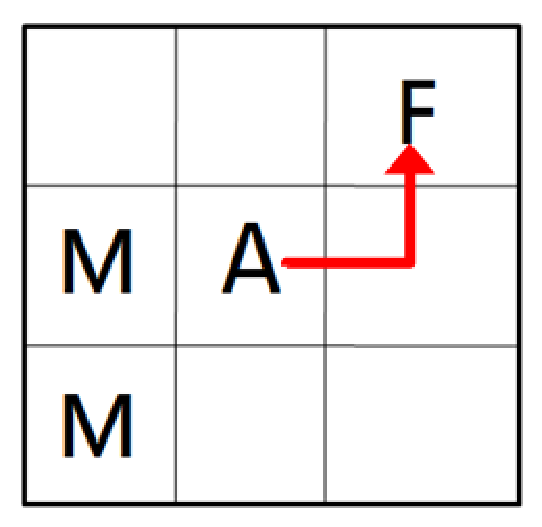
\includegraphics[width=\textwidth] {./figures/monster_plan.eps}
    \end{minipage}
    \caption{The shortest path from the agent's location to the food}
    \label{fig:monster_plan}
\end{figure}
Consider the eat-food-and-avoid-monster game in Fig. \ref{fig:monster_plan}. If the monsters do not move and the actions are deterministic
, the optimal policy of the game can be founded by the shortest path algorithm. The goal state is the location of the food,
the cost to move to the adjacent location is $1$, if there is a monster in the adjacent location, the cost 
to move to it is $\infty$. The agent only needs to compute the lowest cost path from its current position to the goal,
and choose the action which can keep it on this precomputed path.

However, the game is not a static one. The monsters may move around and block the precomputed path. The actions of
agent may have unpredictable result to lead it out of the precomputed path.
This stochastic natural of the game makes it natural to formulate the problem as a stochastic shortest path
problem. A stochastic shortest-path (SSP) problem is a MDP problem with a absorbing goal state and positive costs.
A solution of a SSP problem is a policy from the initial state to the goal state with minimum expected cost.

A work by Zucker et al. \cite{Planner} introduced a two-level approach to solve a maze problem.
The planner uses the shortest path algorithm to find a path from the current state to the goal state.
The cost of each step is estimated by Q value, which is computed by the SARSA algorithm.

A issue occurred when we want to apply this approach to general MDP problems: we do not know the 
goal state. The objective of MDP is to find a sequence of actions which can maximize the overall 
rewards. There are no clearly defined "goal" for the MDP problems.

A possible way to adopt the planning technique to the MDP problems is to choose a sequence 
of goals which can maximize the overall rewards. The goal can be chosen to be the state
with the highest expected reward. To achieve this, an agent needs to learn 
the probability to move from one state to another, and the reward to be received
from each state. 

The approach is two fold. In the beginning, the planner selects a path from the current 
state to the goal state with the highest expected reward. The path consists of several
nodes, which are considered as the subgoals of the plan. The RL agent finds the subgoal 
right after the current state, and chooses a sequence of actions which can lead the agent
to the subgoal. The result can be either success or failure, and the probability of the successful
rate of a plan would be updated accordingly. The planner then use the updated information to 
compute a new path.


%application: the key-room problem--> each room lock a key, one room has a treasure, the agent needs to go through 
%a maze to collect the keys for each door and get the treasure

%Stochastic Shortest-Path Problems
%A Stochastic Shortest-Path problem is an mdp prob-
%lem in which the state space S = f1; : : : ; n; tg is such
%that t is a goal (target) state that is absorbing (i.e.,
%p(t; u; t) = 1 and g(t; u) = 0 for all u 2 U(t)), and the
%discount factor ® = 1. In this case, the existence of
%optimal policies (and optimal stationary policies) is a
%major mathematical problem. However, the existence
%is guarantee under the following reasonable conditions:
%(A1) There exists a policy that achieves the goal with
%probability 1 from any starting state.
%(A2) All costs are positive.
%The ¯rst assumption just expresses the fact that the
%problem admits a well-behaved solution. Such policies
%are known as proper policies. The second assumption,
%in the other hand, guarantees that all improper policies
%incurs in in¯nite cost for at least one state. Thus, both
%assumptions preclude cases where the optimal solution
%might \wander" around without never getting to the
%goal. For example, a problem having a zero-cost cycle
%(in state space) violates the second assumption.
%As mentioned in the Introduction, often we are only
%interested in knowing how to go from a ¯xed initial
%state, say 1, to the goal state. The optimal solution in
%this case is an partial optimal stationary policy ¹ such
%that ¹(i) = ¹¤(i) for all states i that are reachable
%from 1 when using the optimal policy ¹¤; the so-called
%relevant states when starting from 1.1
%Finding a partial optimal policy can be consider-
%ably simpler, the extreme case when the set of relevant
%states is ¯nite and the complete state space is in¯nite.
%Thus, the question of how to ¯nd partial optimal poli-
%cies is of great relevance. One algorithm for that is
%Real-Time Dynamic Programming.


%TODO: add maze problem with invisible trap as illustration for transfer learning, so the location of trap is important. Otherwise, the learning rate may decrease.
%TODO: show that bus domain is an example for delayed death.

\chapter{Empirical study}

In this chapter, we demonstrate the effectiveness of our approach in the 
Bus and Infinite Mario domains.
The Bus domain is a 6 by 6 grid world problem. 
We have $2304$ states in this domain, so it is small enough to apply table-lookup methods to learn
the optimal policy. In this experiment, we combine table-lookup HORDQ and an approximate model-based method 
to illustrate how to increase the learning rate and learn a near-optimal policy with our approach.

For large problems with more than millions of states, it is not possible to use table-lookup methods to learn the optimal policy.
Instead, it is necessary to adopt function approximation techniques to learn the policy.
However, the optimality guarantee of Theorem \ref{thm:opt} relies on table-lookup methods and 
does not hold for function approximation techniques.
With function approximation, it is not possible to learn the optimal policy anymore.
We illustrate our work with Infinite Mario to show that despite the fact that the optimality guarantee is lost in
large problems, we can still use model-free methods to help model-based methods handle the effects which
are not included in the model. 
%Since both model-free and model-based methods may not learn the optimal policy, it is possible to 
%combine both methods to learn a better one.

%TODO: why not classical planning?
%TODO: Why it is bad to put too much information to the model?
%TODO: why it is bad to put pit information?


%TODO: Say how do we update the model (just for three iteration) with Bellman equation
%TODO: say we use MaxQ for model based approach
\section{Bus domain}
\label{se:domain}

\begin{figure}[t]
 \begin{minipage}[b]{0.5\linewidth}
    \begin{center}
    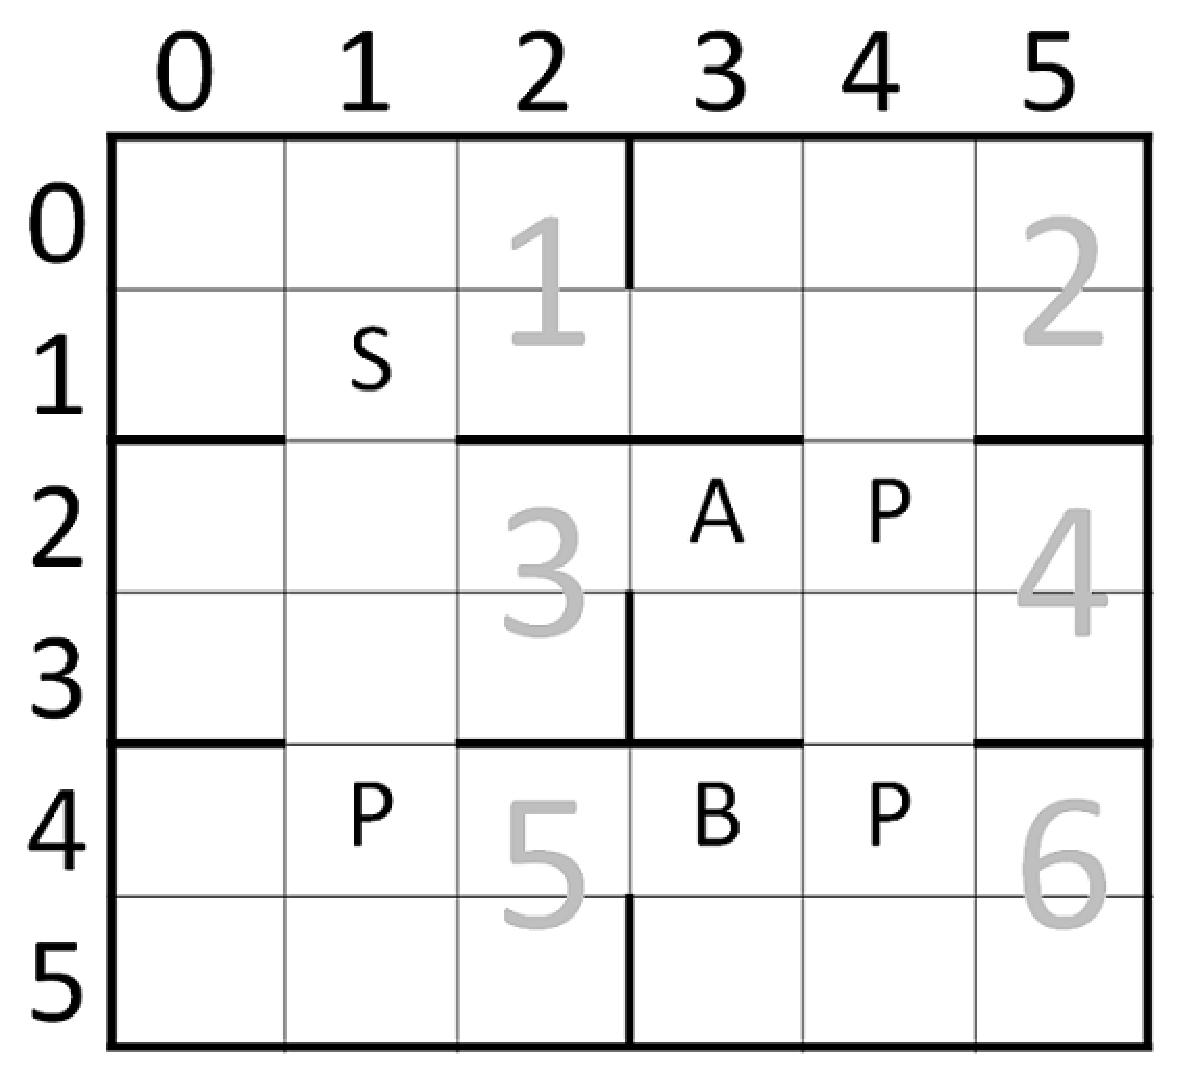
\includegraphics[width=2.0in] {./figures/BusSmall.eps}
\end{center}
\end{minipage}
\begin{minipage}[b]{0.5\linewidth}
    \begin{center}
    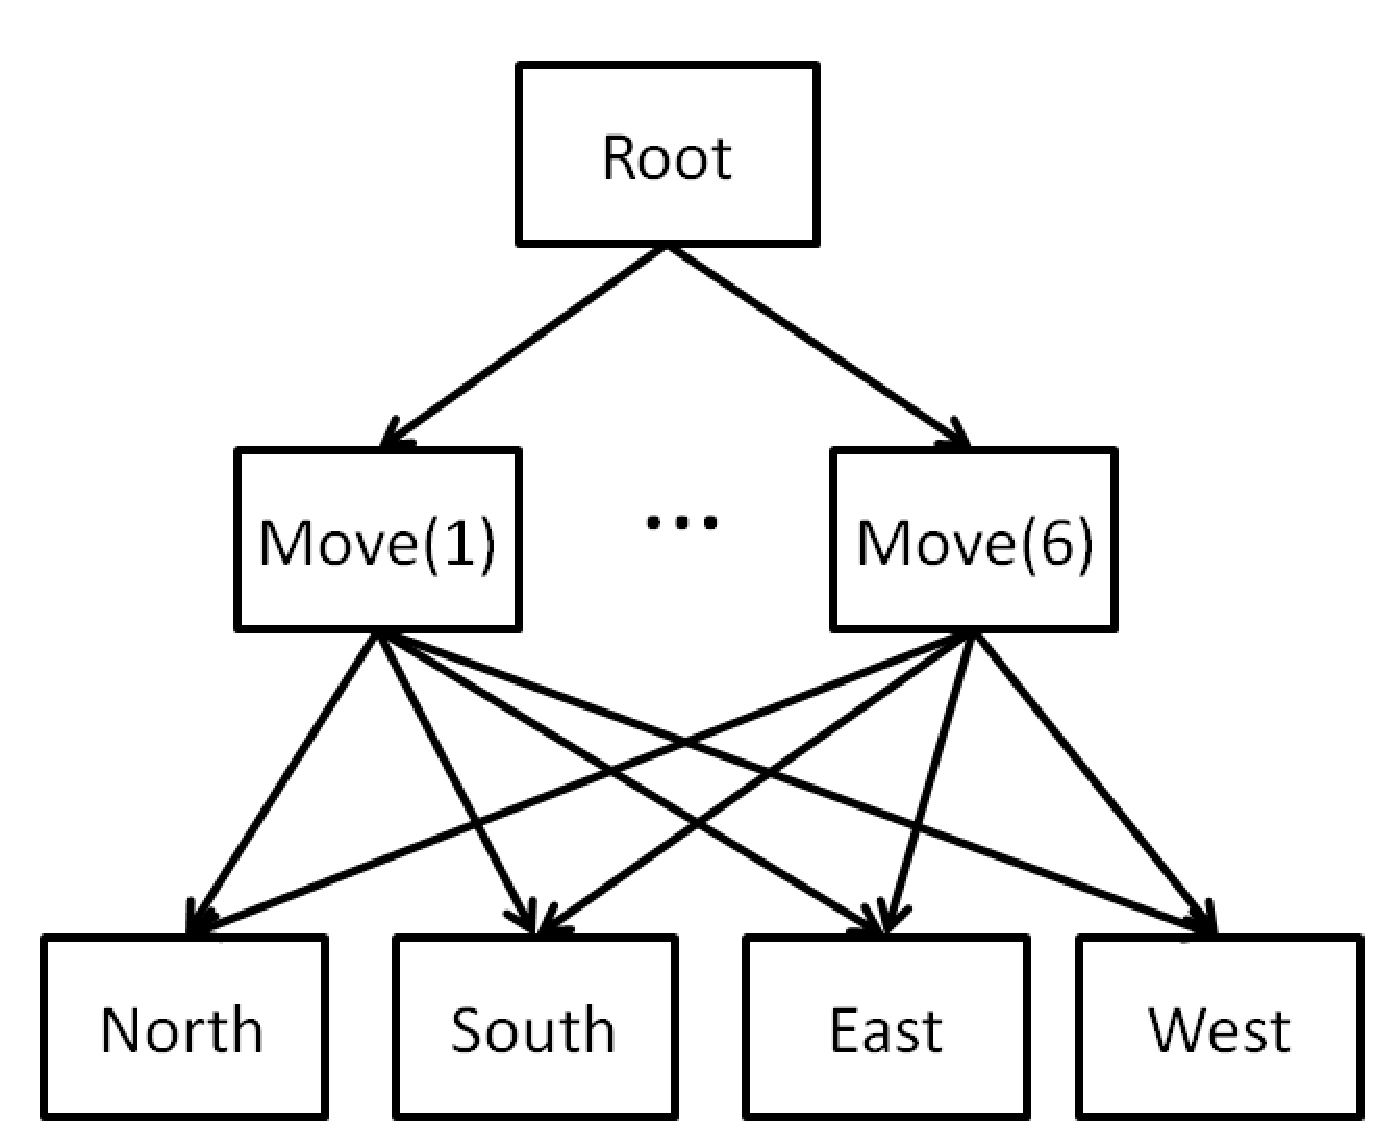
\includegraphics[width=2.0in] {./figures/BusHierarchy.eps}
\end{center}
\end{minipage}
\begin{minipage}[b]{0.5\linewidth} \centering (a) \end{minipage}
\begin{minipage}[b]{0.5\linewidth} \centering (b) \end{minipage}

\caption{(a) The Bus domain (b) A task graph for the Bus domain.}
\label{fig:bus}
\end{figure}

Figure \ref{fig:bus}(a) shows the bus domain. The bus starts at $S$. Its task
is to pickup all passengers marked as $P$ and return to $S$.
The bus can move North, South, East, or West. There is a reward of -1 applied for each action.
There is a $0.1$ probability for the bus to move in a random direction. It stays put 
when trying to cross a wall. 
The passengers are picked up automatically when the bus moves into
the location of a passenger. The passengers can be picked up in any order.
The episode ends when it finishes the task.  
There are two possible locations for road construction. They are marked as 
$A$ and $B$. If the bus passes a construction site, it will get damaged with probability 1 and has the probability
of 0.25 of breaking down for each step afterwards. There is a reward of $-50$ if the bus breaks down and the episode ends immediately. 
At the beginning of an episode, the status of the road is randomly chosen from no construction, $A$ is under construction,
or $B$ is under construction. There is a $0.05$ probability for the road status to change for each step.
The world is divided into six areas. There are six subtasks $Move(1), \dots,$ and $Move(6)$ which move the
bus to the corresponding area.
Subtask $Move(t)$ can only be invoked if $t$ is the adjacent area.
The subtask terminates if the bus exits the current area.
When it terminates, a pseudo-reward is applied if the bus arrives at designated area $t$ and 0 otherwise.
The task hierarchy is shown in Figure \ref{fig:bus}(b). 

A state can be described by a 8-tuple $(x, y, h, p_1, p_2, p_3, a, b)$, where $(x, y)$ is the location of the bus, $h$ shows if the bus is damaged, $p_i$ indicates if the corresponding passenger has been picked up or not,
and $a$ and $b$ are binary variables which indicate the status of the construction sites.

%TODO: the damage status is not perceived on the screen, so it cannot be modeled
Since the six subtasks $Move(1), \dots,$ and $Move(6)$ cover all primitive actions, they form a total leaf cover of the hierarchy.
We used HORDQ in the subtasks to guarantee the convergence to the optimal
policy. Subtask $Root$ adopted our approximate model-based method. 

%The planning variables include 
%the location of bus and the status of passengers. The environment variables are the 
%damage status of bus and the status of road. 
%TODO: total leaf cover always exist
%The world is divided by 6 areas. 

\subsection{Planning with static assumptions}
\label{se:Model}

%We adopted model-based approach 

%TODO: dyanmic programming
%TODO: add free + free HORDQ to show that HORDQ makes the hierarchical process useless
The variables of our model are $\{x, y, p_1, p_2, p_3\}$, while the damage
status and road conditions are assumed to be static during the planning process.
Our model can learn that a large penalty will be received when the bus is damaged.  
However, our model cannot learn that the bus will get damaged if it passes through
a construction site. The model is certainly biased in this case, thus
it cannot learn the optimal policy. The objective of 
the experiment is to show that the optimal policy can still be learned
if we combine the model-based approach with HORDQ. 

%Based on the results of the previous section, we can safely use any approximate model-based method 
%to learn the Q-values of subtasks which do not belong to $TC(H)$ without worrying
%that it will violate the optimality condition. Model-based RL requires the enumeration of all possible states during the planning process.
%However, it is not feasible when the state space is too large.
%Previous methods (\cite{ApproxDyna, ApproxTree}) rely on function approximation
%techniques to predict the next state. Their model is biased because it is possible 
%to encounter different next states given the same state and policy for a stochastic problem. If we 
%predict one of them, we ignore the stochastic nature of the problem. If we predict
%several, the number of states under consideration may grow exponentially with the number of simulating steps
%and become intractable after a few steps.

%We notice that, for some applications, there are some variables which are more important
%than others. Take the mobile robot navigation problem, for example; the location of the robot 
%is the key to the planning process, while the movement of other objects in the environment is less important.
%Our idea is to separate the variables into planning variables 
%and environment variables. During the planning process, we enumerate all possible values of the planning variables, while assuming 
%the remaining environment variables are static throughout the process. 
%If we limit the number of planning variables to be small, the enumeration process can be efficient.
%It also simplifies the learning of the transition and reward functions, since we only need to learn
%the dynamics and reward models for the planning variables.

Let state $s = (x, y)$, where $x$ consists of planning variables and $y$ consists of environment
variables. Following the MAXQ approach, we decompose the Q-function as:
\begin{equation}
    Q^{\pi}(i, x, j) = Q_r^{\pi}(i, x, j) + Q_c^{\pi}(i, x, j),
    \label{eq:biasedMaxQ}
\end{equation}
where $Q_r^{\pi}(i, x, j)$ is provided by the child subtask $M_j$.

The task of subtask $M_i$ is to compute $Q_c^{\pi}(i, x, j)$ by:
\begin{equation}
    Q_c^{\pi}(i, x, j) = \sum_{x'} P_m^{\pi}(x'|s, j)[Q_r^{\pi}(i, x', \pi_i(x')) + Q_c^{\pi}(i, x', \pi_i(x'))],
    \label{eq:biasedQc}
\end{equation}

With the formula above, the Q-values can be computed by dynamic programming.

For simplicity, we use the multi-time model \cite{SMDP} to model the transition function: 
\begin{equation}
    P_m(x|s, j) = \sum^{\infty}_{N=1} \gamma^N P(x, N|s, j).
    \label{eq:multiProb}
\end{equation}

$P_m(x|s, j)$ can be estimated by:
\begin{equation}
    \tilde{P}_m(x|s, j) = (1-\alpha)\tilde{P}_m(x|s, j) + \alpha [ \gamma^N \delta_{x'x}],
    \label{eq:approxP}
\end{equation}
for all $x \in S_i$, where $\delta_{x'x}=1$ if $x' = x$ and is 0 otherwise.

\subsection{Empirical results in the Bus domain}
\label{se:BusRes}
Figure \ref{fig:res}(a) shows the learning curves with different levels of pseudo-rewards.
With pseudo-reward $+60$, it learned a suboptimal policy because
the pseudo-reward is too large to make subtask $Move(t)$ ignore 
the penalty of breakdown. As a result, the subtask followed 
the instruction of its parent too strictly.

On the other hand, if we do not impose any pseudo-reward, 
the optimal policy can be learned, but the learning rate is
slower than SARSA(0) learning. Since subtask $Move(t)$ has no
incentive to follow the instruction of its parent subtask, 
the learning process is similar to SARSA(0) learning 
except it has six different Q-functions to learn (one for each subtask) instead of one.
Thus it takes longer to learn the optimal policy. 

With an appropriate pseudo-reward, we can get a near-optimal policy
while the learning rate is faster than SARSA(0).
Our experiment shows that a pseudo-reward of +5 is enough to make subtask $Move(t)$ follow 
the order of $Root$ in most of the times, but it is not enough for the subtask to ignore
the breakdown penalty. For example, when $Root$ executes $Move(4)$ to move the bus from area 
3 to area 4 and the road at location $A$ is under construction, $Move(4)$ subtask
will learn it is a bad decision with HORDQ.
Instead of moving to area 4, $Move(4)$ may move to area 1 or 5 to avoid
the breakdown penalty. In turn, $Root$ learns that $Move(4)$ cannot be executed in 
such a scenario, thus it will seek an alternative plan if the same scenario
is encountered.

To illustrate the undesirable result when some suboptimal subtasks exist in 
the hierarchy and the MAXQ framework is adopted, we combine our approximate model-based approach
and MAXQ-Q learning in our experiment. The combination learns a suboptimal policy similar to HORDQ with high pseudo-reward. 
Since MAXQ does not estimate the consequence of its action outside its own subtask,
$Move(t)$ will move to area $t$ at any cost. It leads to the frequent damage of the bus.

To simulate the performance of the combination of a poorly-approximated model-based method and 
HORDQ, we replaced our model-based approach with a random policy.
The result is shown in Figure \ref{fig:res}(b). In this case, SARSA(0) has the fastest
learning rate. It takes more time for $Move(t)$ to realize that the policy of $Root$ is bad with higher pseudo rewards.
Nevertheless, it will eventually learn a near-optimal policy.
The combination of random policy and MAXQ presented the worst result.

This result shows that a good approximate model 
can help increase the learning rate with the combination of HORDQ. 
If the model is poor, HORDQ serves as a fail-safe mechanism to keep 
the agent from repeating the same poor policy over and over again.
On the other hand, MAXQ learned a poor policy in both cases.  
This evidence suggests that in order to construct a robust HRL 
algorithm, it is beneficial to incorporate HORDQ in the hierarchy.

\begin{figure}[b]
%\begin{center}
 \begin{minipage}[b]{0.9\linewidth}
     \begin{center}
    %\includegraphics[height=11em, width=6em]{eli_bend.eps}
    \includegraphics[width=3.5in] {./figures/Approx.eps}
\end{center}
    %\caption{(a)}
\end{minipage}
\begin{minipage}[b]{0.9\linewidth} \centering (a) \end{minipage}
\begin{minipage}[b]{0.9\linewidth}
     \begin{center}
    \includegraphics[width=3.5in] {./figures/Random.eps}
\end{center}
\end{minipage}
\begin{minipage}[b]{0.9\linewidth} \centering (b) \end{minipage}
%\end{center}
\caption{The learning curve for the bus domain, averaged over 400 episodes. (a) With our model-based approach. (b) With random policy.
The pseudo-reward is shown in parentheses. The parameters are $\alpha=0.1$ and $\gamma=1$. All algorithms follow an $\epsilon$-greedy exploration policy
with $\epsilon = 0.1$.}
\label{fig:res}
\end{figure}


\vfill
\clearpage

%\newpage
%TODO:
%The above experiment assumes the agent knows when
%it will receive the delayed reward.
%However, it 
%It is not a p

%On the contrary, the combination of MAXQ and a poor approximated model has
%a performance similar to random policy.

%TODO: add random agent experiment
%TODO: if I set the pseudo reward to zero, will the whole stuff breaks down again?


\section{Infinite Mario}
\label{se:MarioExp}
%reward system here
%and pseudo reward
We use Infinite Mario to show the effectiveness of our approach in large domains. 
Large domains contain more than millions of states, so it makes table-lookup methods not applicable
due to the curse of dimensionality. Approximation techniques are required to handle these
problems, but the optimality guarantee will be lost.
It is interesting to see how our work will perform with function approximation techniques,
especially when model-free methods cannot learn the optimal policy.

\subsection{Previous work}
Infinite Mario is an open source Java implementation of Nintendo's Super Mario Brothers game.
It received much attention in the AI community possibly due to
the two AI competitions -- RL 2009 competition\footnote{http://2009.rl-competition.org/}
and Mario AI competition\footnote{http://julian.togelius.com/mariocompetition2009/}, which were held in 2009.
The objective of these competitions is to build the best agent that
can play this classic side-scrolling arcade-style game.

%Bruno In the paragraph above, perhaps you could cite the competitions, at least as a footnote directing to their web site
%James added

The RL 2009 competition required competitors to use RL algorithms to build their agents.
On the other hand, the Mario AI 2009 competition \cite{Robin09} 
did not pose any restrictions on the underlying technique.
It encouraged
competitors to use neural networks, genetic genetic programming, fuzzy logic, temporal difference learning, and human ingenuity.

The observation of Mario AI in RL 2009 competition 
contains the location and speed of Mario and other monsters, as well as
the $22 \times 16$ tiles on the screen.
The agent receives +100 reward when it finishes a level, +1 reward when collects
a coin, and -10 reward when it dies.

%Since this competition focuses on RL algorithms,
%the agent needs to learn the property of environment through interaction.

Mohan and Laird \cite{Mohan09} combined HRL and Soar-RL \cite{Nason05} to build
a Mario agent. In their hierarchy, the task is divided to "Grab Coin", "Search Question", "Tackle Monster",
"Avoid Pit", and "Move to Goal". 
The root subtask chooses one of these subtasks to execute based on the learned
preferences. Each subtask deals with at most one object. For example, the
"Grab Coin" subtask is considered successful only when the specified 
coin is collected. Thus, the number of subtasks available for the root task to choose
depends on the current objects in the screen.

Gibson and Risk \cite{Gibson09} adopts the options framework.
The master agent can execute 3 options -- a $SARSA(\lambda)$ agent, a "pit specialist" agent, and a
rule-based agent. The "pit specialist" concerns only with the pits, and is available only when
there is a pit within 4 tiles of Mario. 
The master agent uses SMDP Q-learning to learn which option to execute given a state.

Ringstad et al. \cite{Paul09} 
used a modified linear SARSA algorithm to build the agent.
The input features are the locations of the 3 nearest monsters or pits.
Their idea is to design an agent that can finish the level as fast as possible.
To encourage the agent to finish the level, they rewarded the agent when it traverses
intervals of 10 tiles away from the start.
Their method won the Mario AI championship of RL competition 2009.

%Bruno What is a pseudo-reward? And shouldn't you be describing these contributions in the related work section of your thesis? Possibly in a separate chapter?
%James The reference of pseudo-reward has been removed.
%James It is good question. My concern is that the related work presented here is only related to Mario experiment. Where should I put it?

The state observation of Mario AI 2009 competition \cite{Robin09} includes $22 \times 22$ tiles on the screen, the location and the speed of monsters, 
and the status of Mario such as "isMarioOnGround" or "mayMarioJump".

%Bruno What do these status variables have in common? Are there others? How many variables are there? What's the # of dimensions in the state?

%Booleans: mario is on the ground, may
%jump, is carrying a shell, is small/big/fireprovides an interface
The techniques which are adopted by the competitors of Mario AI competition include
$A^*$ search, genetic programming, hand-coded policy, a hybrid method of neural network and $A^*$ search,
and Cyberneurons.
In general, $A^*$ search achieves the best result, and hand-coded policy falls the second.
Robin Baumgarten \cite{Robin09} won the championship of the Mario AI competition in 2009.
His idea is to create a physics engine that can accurately predict the next state of Mario, 
and use $A^*$ search to find a path to the right border of the screen as fast as possible.
Since his approach requires the agent to have the complete knowledge of the environment,
the approach falls into the category of classical planning.

%Bruno So if classical planning won the competition, either the learning agents were really bad (therefore a bad baseline)
%or the domain is not challenging enough right?
%James Because the classical planning has the complete knowledge of the problem, but RL methods do not.
%James You may that say the domain is not challenging, since we do have the complete knowledge of Mario, but it may not be true for other video games.

Ross et al. \cite{Ross11} used supervised learning to learn the direct policy
mapping between input features and the primitive actions. The input features
are $22 \times 22$ tiles around Mario in previous 4 frames, the state of Mario
and the last 6 actions. The tiles include the types of the ground, blocks, and
monsters.  The state of Mario includes the types (small, big and fire Mario) as well as a
binary feature to indicate if Mario touches the ground or not.
The training data is obtained through search-based methods similar to Baumgarten's work \cite{Robin09}.


The above approaches either depend on game-specific information ("isMarioOnGround")
or depend on the information that is difficult to be retrieved from image features (the location and size of pits).
In this section, we introduce an approach 
of building an agent for Infinite Mario 
without using such information.
We only restrict the agent to use the features provided by the simulator of Infinite Mario from RL competition 2009.
The features can be retrieved from the screen directly, 
therefore it allow us to generalize our approach to other video games without
the need to redesign specialized features for each individual problem.

%Our goal
%is to train the computer to play this game based on the current
%game image features as input (see Figure 3).

%why RL competion is pure image based
%We do not reguire the agent to have prior knowledge about some special tile patterns which are game-specific

%to allow the agent to simulate its own action in the environment that is identical
%to the game itself. It allows people to use the techniques in classical planning,
%such as search-based methods. 

%Infinite Mario, a Java implementation of Nintendo's Super Mario Bros. game, becomes
%a recent interest in the AI community.
%There is also a recent interest in developing agents that can play a complete side-scrolling
%arcade-style game. In 2009, two AI competitions were organized on agents that can play
%entire levels of Inite Mario, a clone of Nintendo's popular Super Mario Bros game. The
%RL 2009 Competition [Mohan and Laird, 2009] requires the agents to use reinforcement
%learning to learn to play the game. The learning agents are given a state representation
%containing the location of the player character (PC) and other monsters, as well as the types
%of the individual tiles on the screen. The agents receive a positive reward once the level is
%complete, and a small negative reward on all other states. The Mario AI Competition4, on
%the other hand, does not limit the agents to a speci approach. Indeed, the participants
%are encouraged to use evolutionary neural networks, genetic programming, fuzzy logic,
%temporal dirence learning, human ingenuity, [and] hybrids of the above"5. Playing an
%Atari 2600 game was previously attempted by Diuk et. al., who illustrated the performance
%of their Object-Oriented Rmax algorithm by teaching the Player Character to pass the st
%screen of the game Pitfall [Diuk et al., 2008].
%A shared characteristic between all the above examples, and (to our knowledge) all
%previous attempts of learning to play video games, is that each agent is designed and tuned
%to play a single game. Therefore, all the essential game properties (e.g., the location of the
%PC and important NPC's, health levels, and timers) are either explicitly included in the
%state representation, or can be easily extracted form it. Also, game-speci abstractions are
%often performed to deal with the large state-space. Furthermore, the reward signal may be
%shaped in a way to accelerate the learning.
%One of the key distinctions of the methods described in this thesis is their generic nature.

%Screen feature
%assume the location of PC is known
%the result is unknown (the properties of monsters or coins)

\subsection{Infinite Mario domain}

We use the 2009 RL competition environment to conduct our experiment.
The action space of Infinite Mario consists of 4 buttons which correspond
to the original Nintendo controller.
These buttons are:
\begin{itemize}
%\item Handle the interaction between objects
%\item Not everything can be modeled
\item Direction pad: left or right
\item A button: jump
\item B button: speed
\end{itemize}
Mario can choose to press these buttons or not, so
the number of possible actions are $3 \times 2 \times 2 = 12$ actions.  

We exclude action "speed", "jump speed" and "no op" from the 
action space, since they do not seem to be relevant to the optimal policy.
The agent can execute 9 actions in our experiment.

%Bruno At this point you could say already if something belongs to the optimal policy or not, since you claim that your method learns this policy right?
%James In Mario domain, it is not clear what the optimal policy is, due to the huge state space.
%James Do you suggest me rephrase it?

The screen of Infinite Mario is comprised of a matrix of $22 \times 16$ tiles.
The matrix is an array of characters, with each element representing the type of tile.
The types of tile are brick, question-block, coin, pipe, empty tile, the finish line and Mario.

Besides the tile information, the information of moving objects are also provided. 
The moving objects are Mario, Red Koopa, Green Koopa, Goomba, Spikey, Piranha Plant, Mushroom, Shell, Fire Flower and Fireball.
The information of each object includes x- and y-positions, x- and y-velocities, and type of object.
Note that the positions and velocities are continuous, so a quantization technique might be required.

The tile information can be captured from screen with basic image processing techniques \cite{Yavar}.
The location and speed of monsters can be obtained by applying computer vision techniques such
as object tracking or optical flow.

The levels are generated with 3 parameters: random seed, type, and difficulty.
The difficulty ranges from 0 (easiest) to 9 (hardest). 

The agent will receive the following rewards:
\begin{itemize}
%\item Handle the interaction between objects
%\item Not everything can be modeled
\item +100: finishing a level
\item +1: collecting a coin
\item +1 : hitting a question block
\item +1 : killing a monster
\item -0.01 : step cost
\item -50 : getting killed
\end{itemize}

Besides, we apply a reward equal to the
displacement of x-position to encourage the agent to move as right as possible
and penalize the agent if it moves to left.

%Bruno Where this choice come from? Would your method work without it?
%James Because Mario doesn't know the exit is at the far end of his right, it needs some motivation to move in that direction.
%James So no method will work without it.

\subsection{The model-based method for Mario domain}
%TODO: only 9 actions
%TODO: sampling

\begin{figure}[t]
 \begin{minipage}[b]{0.45\linewidth}
    \begin{center}
    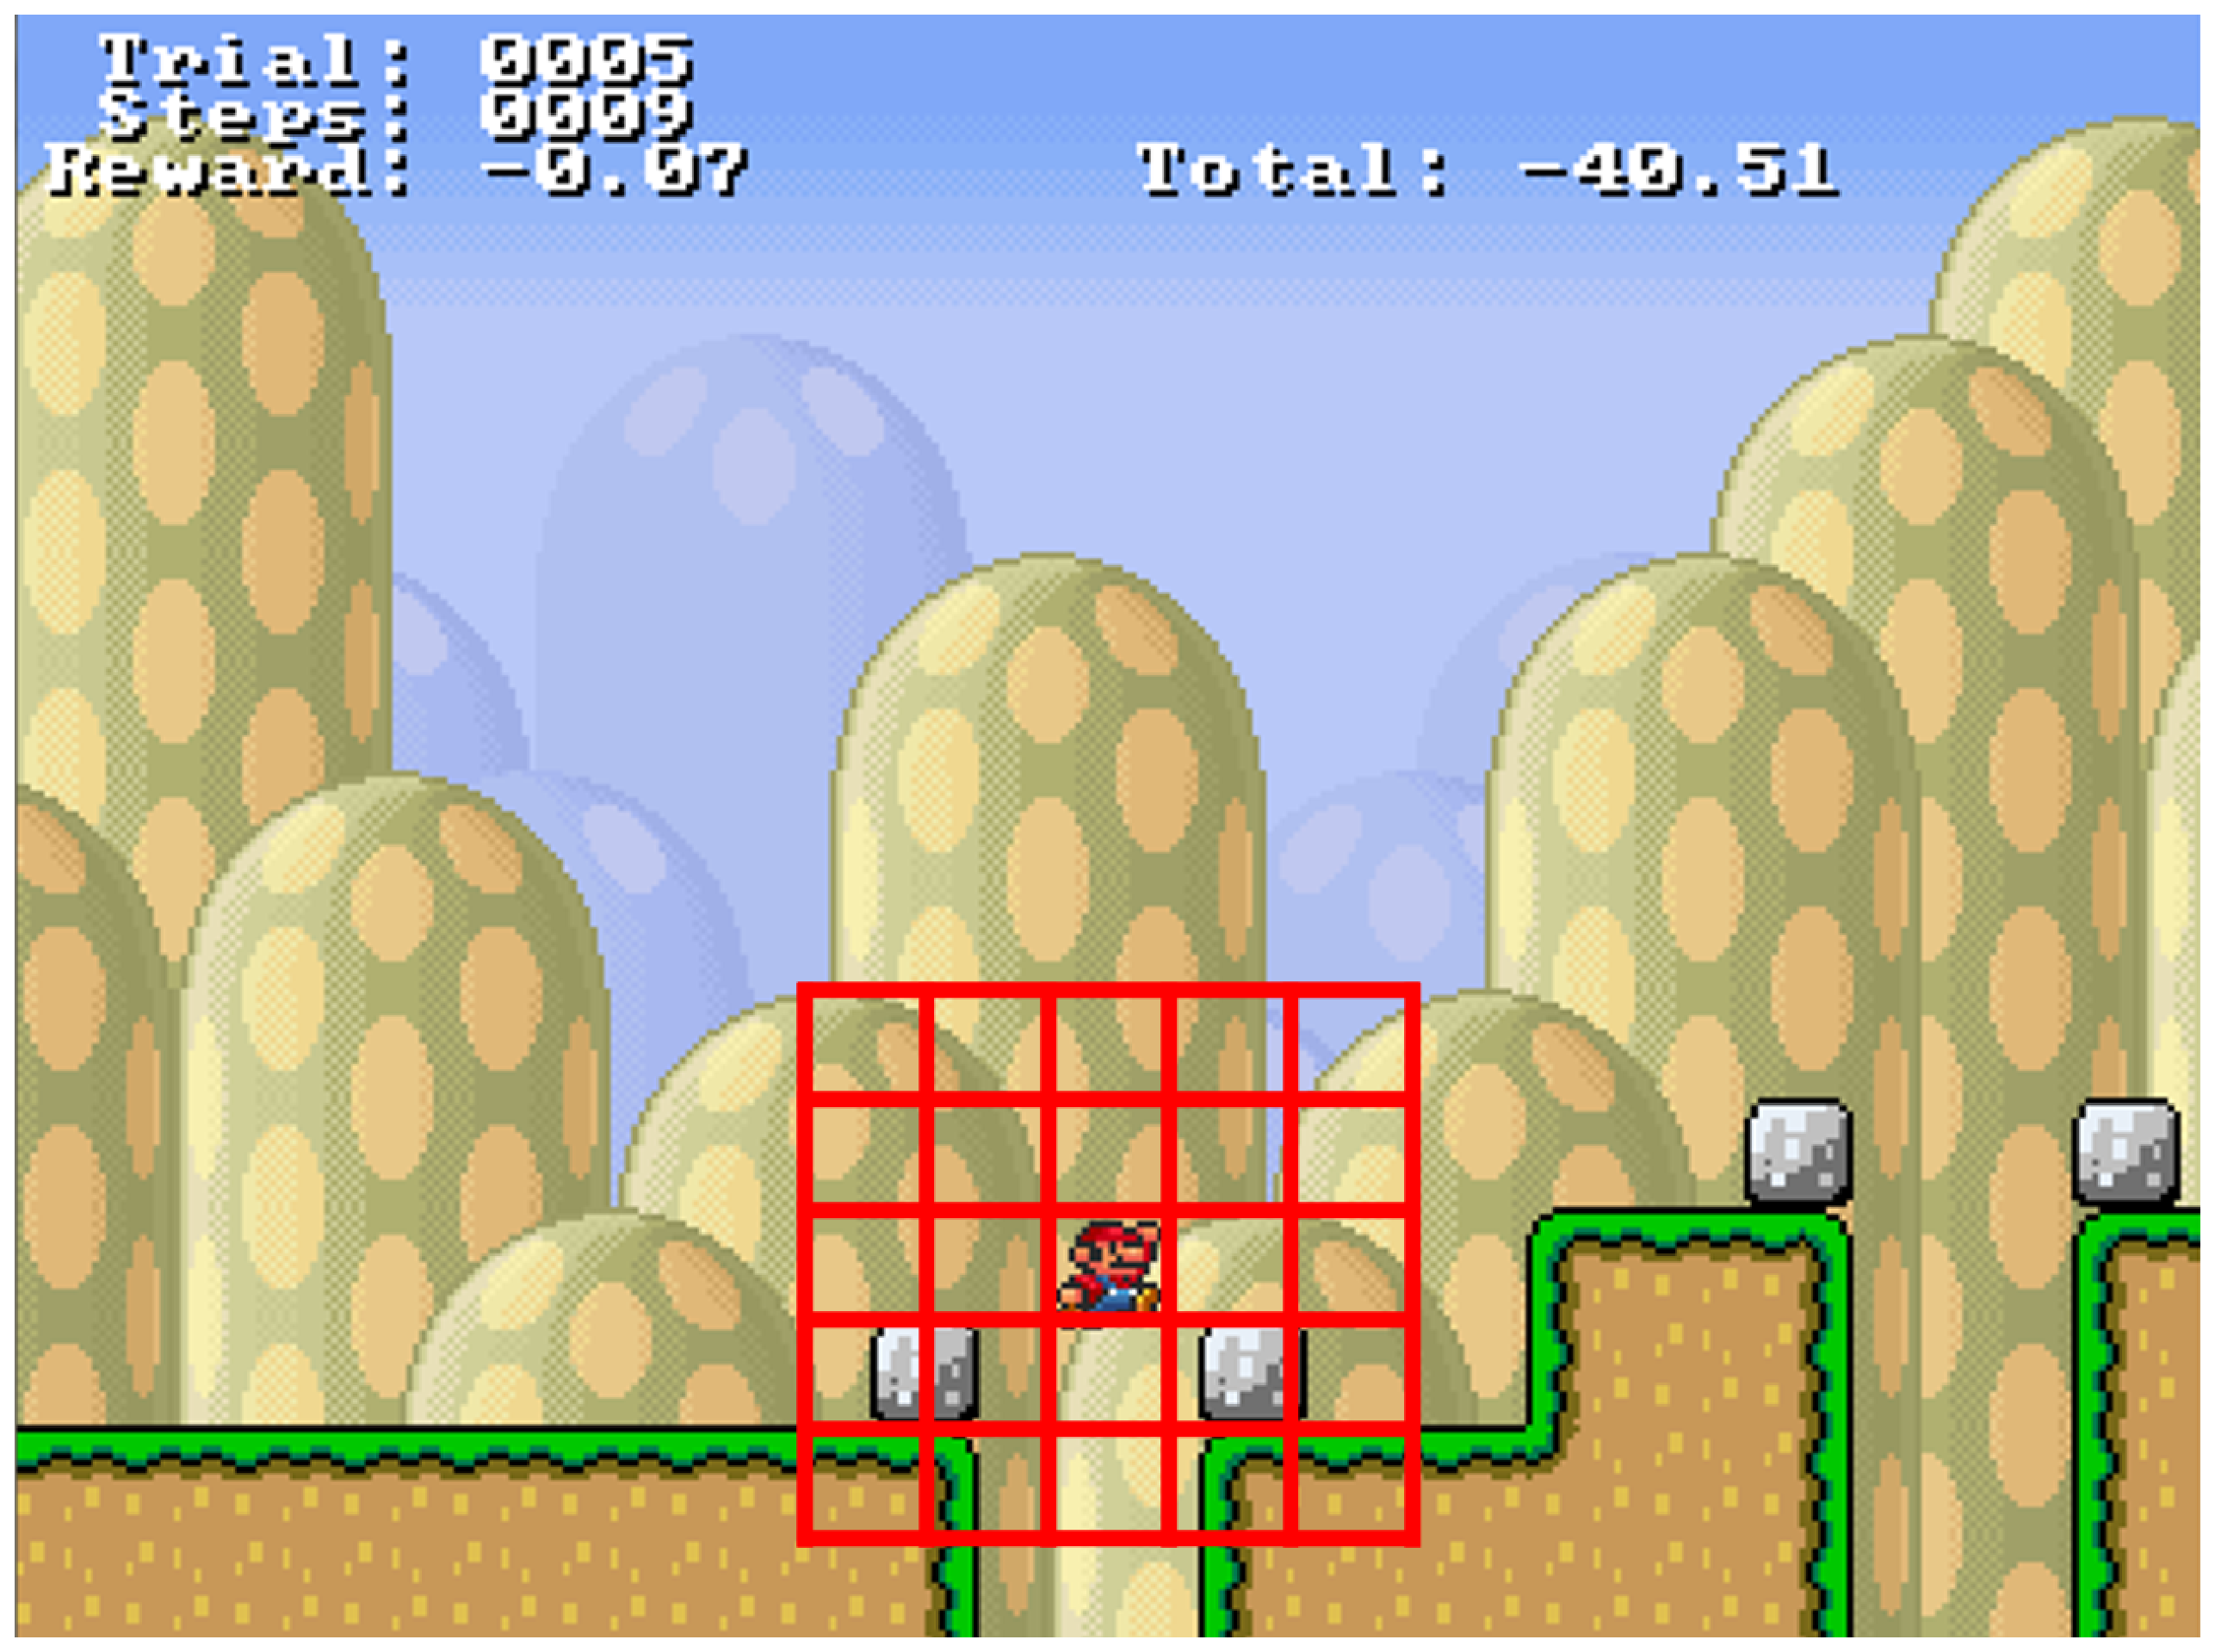
\includegraphics[width=2.0in] {./figures/MarioGrid.eps}
\end{center}
\end{minipage}
\begin{minipage}[b]{0.45\linewidth}
    \begin{center}
    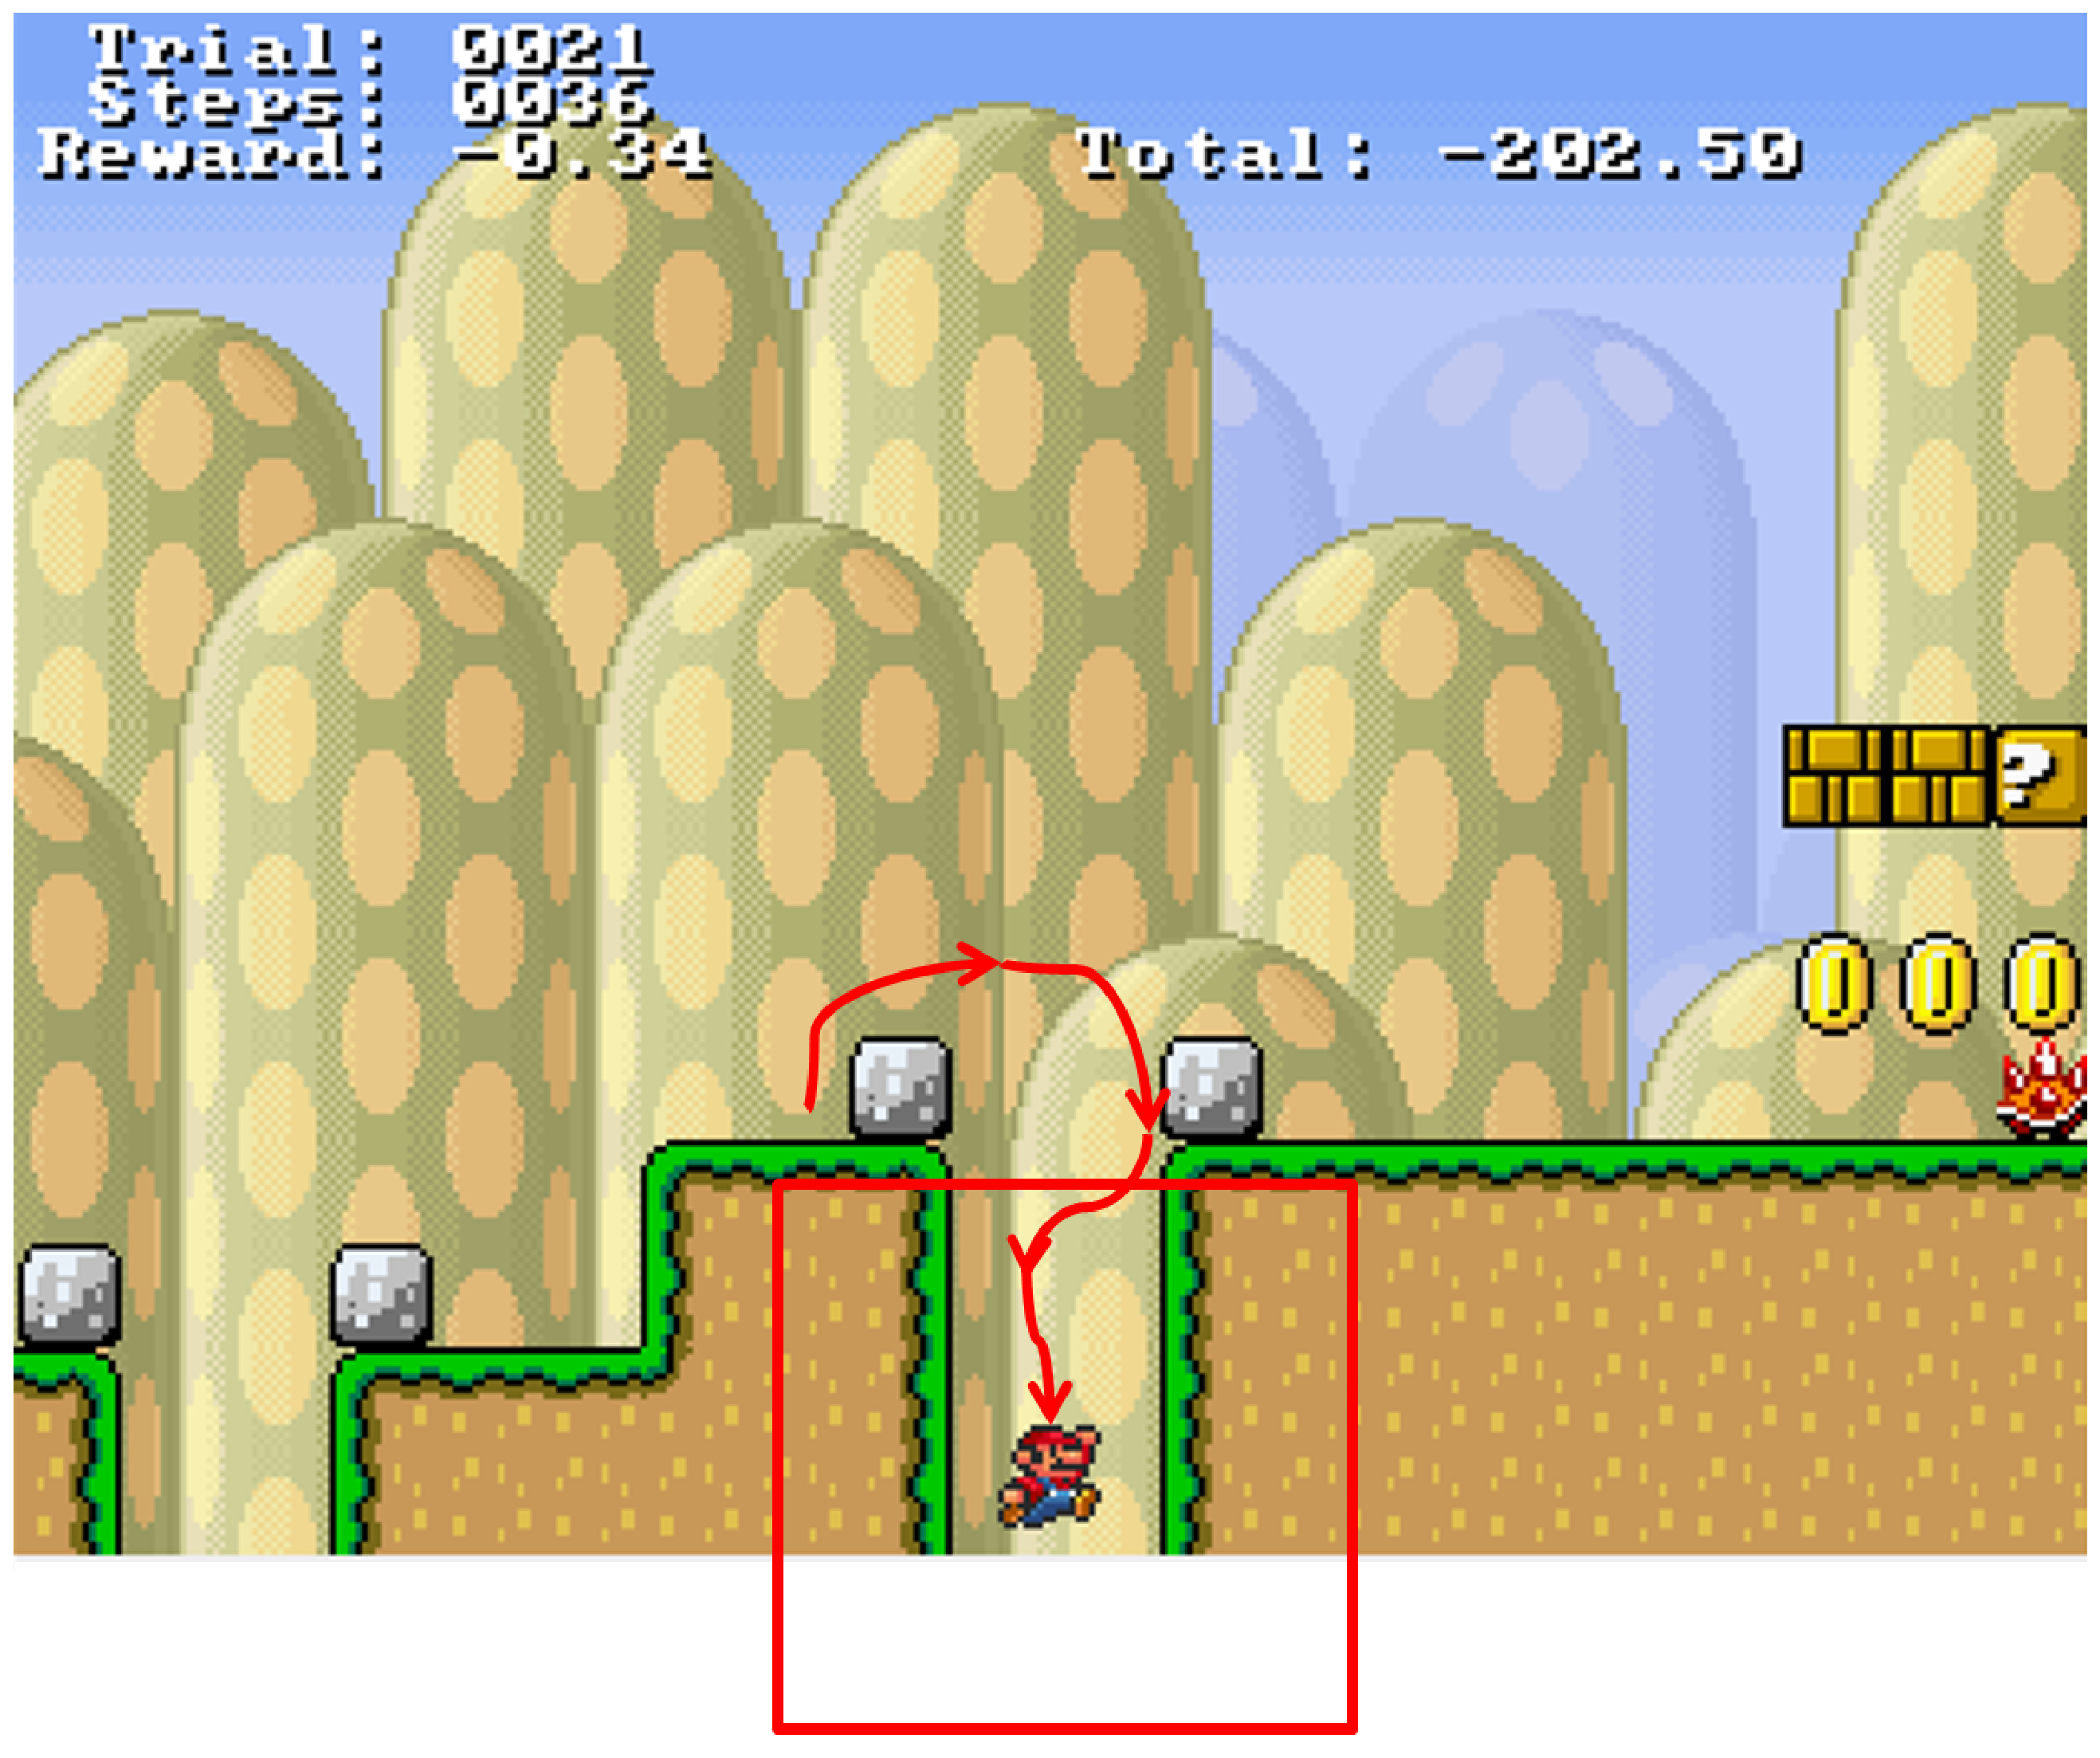
\includegraphics[width=2.0in] {./figures/MarioModel.eps}
\end{center}
\end{minipage}
\begin{minipage}[b]{0.45\linewidth} \centering (a) \end{minipage}
\begin{minipage}[b]{0.45\linewidth} \centering (b) \end{minipage}

\caption{(a) A screenshot of Infinite Mario (b) A planning process conducted by the search-based method.}
\label{fig:Mario}
\end{figure}

%We adopt greedy search in our planning process.
%The planning process begins with a state of Mario. 
%Then it iteratively acquires the next states by applying
%the 9 actions to the state. To avoid fully expand the whole search tree to 
%the depth $K$, which is time-consuming and unnecessary, we expand the state

We adopt the model-based method to learn the transition function of Mario.
The state of Mario 
can be described by a 4-tuple $(x, y, dx, dy)$, where are the location and velocities of Mario. 
The ranges of $x$, $y$, $dx$ and $dy$ are $[0, 318]$, $[0, 15]$, $[-2.5, 2.5]$, and $[-2.5, 2.5]$.
These variable are continuous, so it is not possible to enumerate all possible states
of Mario with dynamic programming techniques. It is possible to discretize the variables, but the resulting state space 
would still be too large if we want to predict the dynamics of Mario precisely.

Instead of discretizing the variables, we used the regression tree algorithm
in the Orange package \cite{Orange04} to predict the future position and speed of Mario.
The features are the current speed of Mario and the tiles within 5 by 5 
area around Mario (Fig. \ref{fig:Mario}(a)). There are 27 variables. 
Since each action has different dynamics, 
we build different trees for different actions. 
Given the current state and action, the regression trees should predict 
the speed and position of the following state. 
The regression trees predict
the relative changes of positions $\epsilon_x = x' - x$ and 
$\epsilon_y = y' - y$ since modeling relative change might generalize better across states \cite{Hester09}.
However, the relative changes of speeds do not generalize well, so we predict
the value of speeds directly.
%(a possible reason is that the maximum speed is capped, so Mario cannot
%keep increasing its speed by press the speed button). 
The x-position, y-position, x-speed and y-speed are the class variables for the regression trees.
For simplicity, we separately build regression trees for different class variables and actions. 
In our current implementation, there are 9 actions and 4 class variables, so we 
have 36 regression trees to model the dynamics of Mario. 

We borrowed the idea of Baumgarten \cite{Robin09}, using
the search-based method to find a sequence of actions that moves Mario to the right edge of the screen as fast as possible.
Instead of hard-coding the objective of the search process, we add a possible reward to the agent if it moves
to the right and a negative reward otherwise.
We adopt a simple k-step lookahead greedy search in our planning process.
It begins with the current state of Mario. 
Then it expands one node in the search tree by applying all possible actions. 
To avoid fully expanding the whole search tree to 
the maximum depth, which is 6 in our experiment, we use greedy search and expand the node
with the largest predicted reward. 
The process stops after the number of nodes exceeds 300, then the search algorithm returns 
a sequence of actions which achieves the highest predicted reward.
To reduce the computation time spent on searching, the search algorithm will return
immediately if there is a sequence of action which gets more than +6 reward.
There are $9^6=531,441$ nodes in the fully-expanded tree. 
Since we only search a very small part of it, it is possible for the search algorithm
to return a suboptimal sequence.
The locations of monsters and other objects are assumed to be the same
during the planning process. 

It is crucial for the search-based method to learn when Mario is going to be killed. 
However, the number of samples right before Mario gets killed is limited by the
number of episodes due to the fact that the episode terminates immediately after the death of Mario.
To efficiently use the available samples, we use a single regression tree to learn the 
reward function. The input features of the regression tree are
the features for the transition function plus the action of the agent. 

The strength of the above method is that it has the terrain knowledge and can move
efficiently to finish a level.
%Another advantage is that it can predict a sequence of actions to jump over a pit.
%The primary difficulty for model-free methods to deal with the pit is that 

%It is quite often that Mario suffers a inevitable death (such as jumps into a monster or falls into a pit).
%If such a scenario happens, there are no actions that can save Mario.
%All action sequences will have a negative predicted reward, so our early return heuristic does not work.

%all possible states of Mario, the planner in our experiment 
%is a $K$-step lookahead greedy search algorithm. The planner searches the states
%which can be reached from the current state within $K$ steps and returns a sequence of
%steps which achieve the highest reward.


%It is crucial for the planning process to learn when Mario is going to be killed. 
%However, the number of samples right before Mario getting killed is limited by the
%number of episodes, which is much smaller than the number of steps. 
%To efficiently use the available samples, we use a single regression tree to learn the 
%reward function.


%To adopt $A^*$ search
%We adopt our static assumption on all objects except Mario. 



%

%TODO: objective: generic AI, challenge here (no specific domain knowledge)
%why model-free approach is necessary

Since we only model the dynamics of Mario, effects such as the dynamics of other objects or
the interactions between objects are ignored. 

Here is the list of effects which are not included in the model:
\begin{itemize}
%\item Handle the interaction between objects
%\item Not everything can be modeled
\item Monsters may appear at the right edge of the screen
\item Monsters disappear at the left edge of the screen
\item Monsters can be killed by Mario, a fireball, or a moving shell
\item Monsters can be killed by falling into a pit
\item Koopma can be turned into a shell
\item Mario can kick a shell to make it move
\item Jump on top of a moving shell will make it stop
\item Fire Mario can attack with fireballs
\item Small Mario can be turned into Big Mario by consuming a mushroom
\item Big Mario can be turned into Fire Mario by consuming a fire flower
\item Coins, mushrooms and fire flowers can be consumed by Mario
\end{itemize}

To learn the transition function perfectly, it is necessary to 
learn all the effects correctly. However, learning the effects for a stochastic
problem is NP-Hard \cite{Walsh09} and heuristic solutions are required
to solve it \cite{Pasula07}.

Our work provides an alternative approach to this problem--instead of learning 
all possible effects, we only learn part of them and 
let model-free methods handle the scenarios associated with
the effects which are not included in the model.

The 5 by 5 tiles around Mario include the monsters as well,
so it is possible for the model-based method to learn the imminent
death caused by moving Mario directly to monsters. What it cannot handle is the delayed death cases, which happen when
Mario moves very close to monsters, but does not touch it.
In such a scenario, it doesn't matter which action Mario is going to take, 
the subsequent death is guaranteed. 
This also happens when Mario moves to a position which will be surrounded by
monsters. After Mario moves to such a position, Mario will be killed inevitably.
%Since there are no way out, the death is inevitable. 
The supervised learning can only learn the reward function with immediate reward.
When the death is actually caused by a decision made few steps before, it is difficult
for a supervised learning algorithm to figure out such a relationship. 
On the other hand, such a delayed feedback will propagate back to previous states with model-free methods
such as $SARSA(\lambda)$, so it is not a problem for these methods.
%The heuristic to reduce the search time
%TODO: up to 6 tiles away
%TODO: no jump involved when it is not going to move up (list all primitive actions, and why they greatly reduce the search space)
%TODO: stop search when is the reward to too negative

%details
%model-based approach knows both tile info and monster info



%The generality of my approach presented here
%If we have a perfect simulator which is identical to the environment, 
%it is possible to use K-step lookahead to find an path from beginning
%to the end (TODO: Mario Competition here). We do 
%conduct the planning process perfectly without 
%resort to 
%It is possible to have a pe

\subsection{The model-free method for Mario domain}

%Bruno Perhaps this section could be called The model-free method and its relation to the problem you illustrated before.
%James Title changed

Since the model-based method cannot deal with the interaction between objects, we use a
model-free method to handle it.

The features of model-free methods include the types and locations of moving objects
other than Mario itself. To reduce the number of features, we do not include the speed of objects.
As noted in \cite{Gibson09}, it is more generalizable if we use "egocentric representation".
That is, we use the relative positions between Mario and objects 
as the features instead of the absolute positions.

Since the number of monsters can be any arbitrary number, 
we cannot use linear SARSA which depends on a fixed feature size.
Instead, we use relational approaches here. 
We incorporated relational temporal difference learning (RTDL) \cite{RRLTD}
with HORDQ. RTDL is a relational extension to linear SARSA, thus it does not
work for continuous variables. To discretize them, we simply
round each variable to the nearest integer. 

Unlike previous approaches \cite{Paul09, Gibson09, Mohan09, Mohan10},
we do not include the location of pits in our features.
Since the pit is not a moving object nor does it occupy a single tile,
it is not available in the input features.
Previous approaches relied on prior knowledge of the shape and size of pits to parse the tile information
and extract the location of a pit. 
We argue that this would not contribute to the generality of the method.
It would be possible to include the pit information by using the whole screen ($22 \times 16$)
as the feature. But the potential huge state space makes it inapplicable in practice ($14^{352}$ states with 14 different types of tiles)
Moreover, it is not necessary to include the pit information in model-free methods,
since the pit can be handled by the model-based method. 

\subsection{The hybrid approach}
\begin{figure}[ht]
 %\begin{minipage}[b]{1.0\linewidth}
    %\begin{center}
    %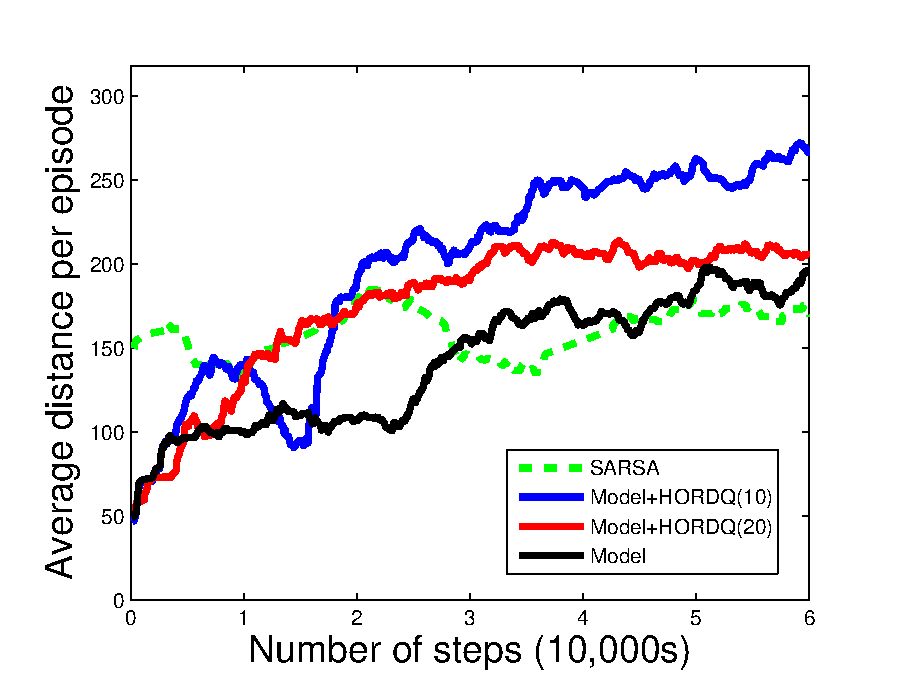
\includegraphics[width=4.0in] {./figures/1247.eps}
%\end{center}
%\end{minipage}
%\begin{minipage}[b]{0.5\linewidth}
    \begin{center}
    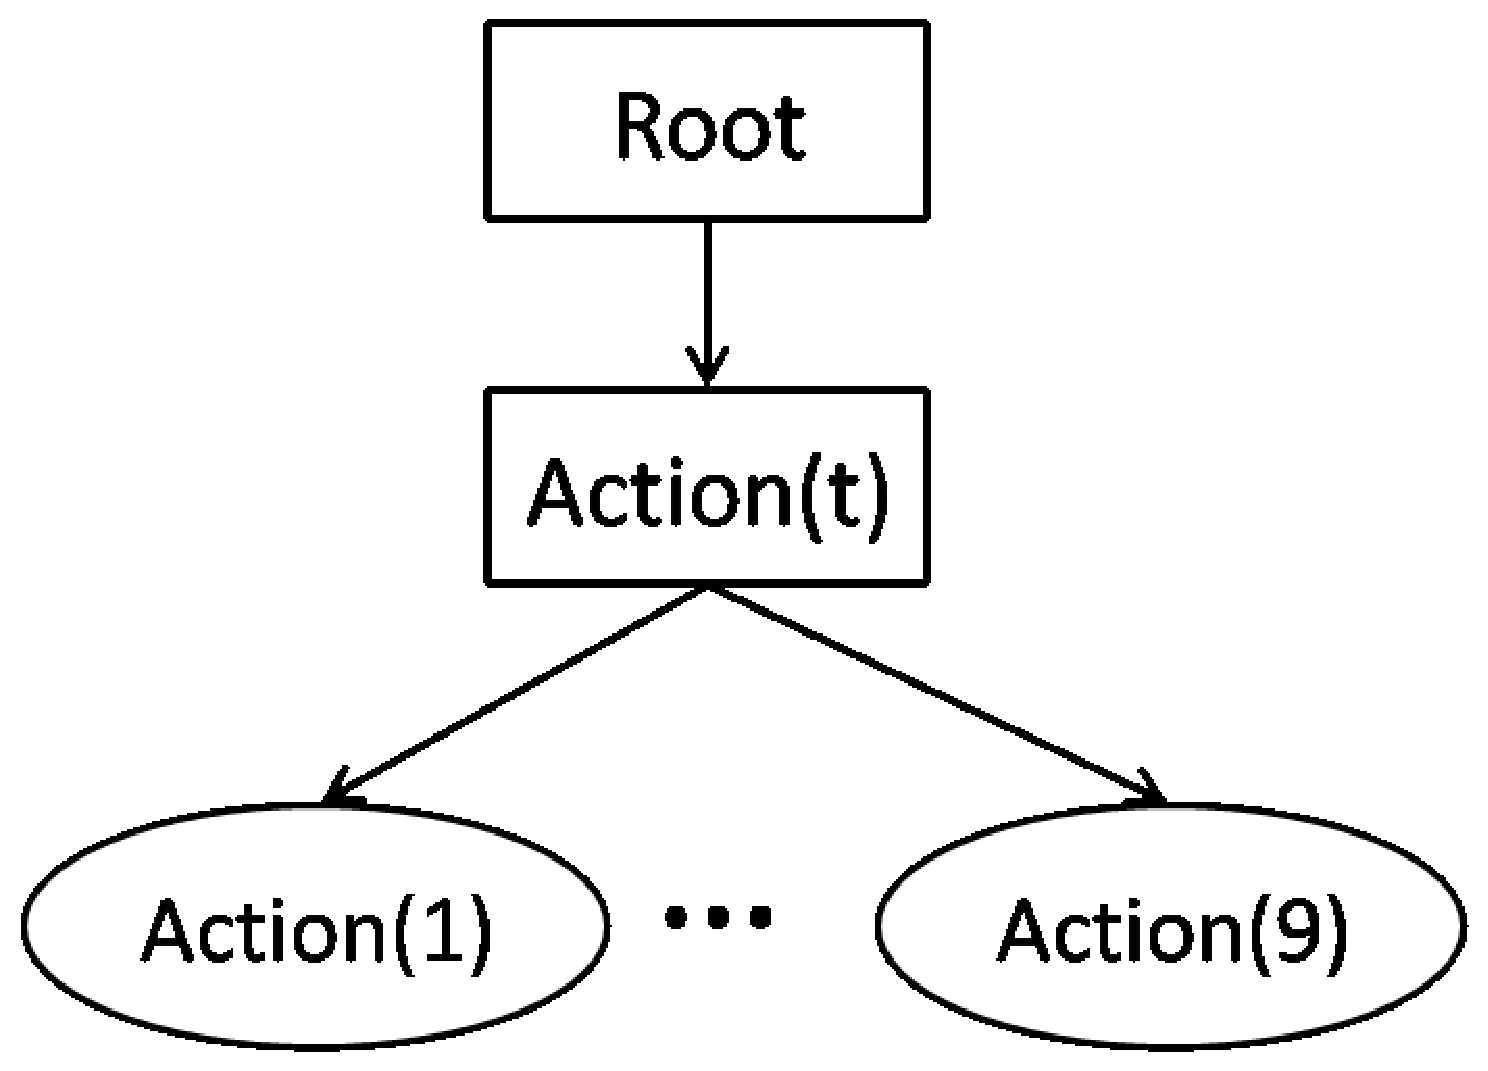
\includegraphics[width=3.0in] {./figures/MarioHierarchy.eps}
    \end{center}
%\end{minipage}
%\begin{minipage}[b]{0.5\linewidth} \centering (a) \end{minipage}
%\begin{minipage}[b]{0.5\linewidth} \centering (b) \end{minipage}

\caption{A task hierarchy for Infinite Mario}
\label{fig:MarioHierarchy}
\end{figure}
We combine the model-based method and model-free method with the task hierarchy shown in Fig. \ref{fig:MarioHierarchy}.
The model-based method is responsible for subtask $Root$ and the model-free method is for
subtask $Action(t)$.
For each step, subtask $Root$ selects one of the actions to execute.
Subtask $Action(t)$ then decide if it is going to follow the action suggested by $Root$ or not. 
If it does, $Action(t)$ will receive a pseudo-reward. 
Since $Action(t)$ is the only subtask that executes the primitive action,
the behaviour of the agent solely depends on its decision.
Subtask $Root$ can only influence its decision with the pseudo-reward.
Note that $Action(t)$ will terminate immediately after executing a single primitive action.
There is no temporal and spatial abstraction in this hierarchy.
That means that we do not enjoy any benefits from adopting the HRL framework.
In fact, the reason we adopted the HRL framework is to combine different methods.
And the benefit of doing so does not come from the HRL framework, but from the power of combining
model-free and model-based methods.

Unlike our approach with the Bus domain, we do not have 
individual subtask $Action(t)$ defined for each primitive action. 
Since subtask $Action(t)$ knows that it will be rewarded if it follows 
the action of $Root$, there is no need for us to separately learn the Q-function for every possible action. 
Instead, we use a single subtask $Action(t)$ to learn the Q-function for the original MDP. 
And the decision of $Action(t)$ is biased with the pseudo-reward when it is going to select the best action to execute. 
Thus, the method presented here does not have the overhead of maintaining multiple Q-functions as in our method for Bus domain.
%For this hierarchy, there is one 

%The state transition function and reward function depend on the policy of 
%child subtask, because the child subtask invoked by $root$ may not correspond to the primitive action that is executed by Mario.
%It would be more difficult if the effects and the policy are learned at the same time. 
%Instead, the transition function is learned from the primitive action that is executed by Mario.

For this special hierarchy, the pseudo-reward imposes a very interesting property:
the policy is identical to the policy of model-free method when a pseudo-reward is equal to zero and
it is identical to the one of model-based method given a sufficiently large pseudo-reward.
We can adjust the value of pseudo-reward to alternate the agent's behaviour between
two different methods.


\subsection{The result of Infinite Mario}
\label{se:MarioRes}
\begin{figure}[t]
 \begin{minipage}[b]{1.0\linewidth}
    \begin{center}
    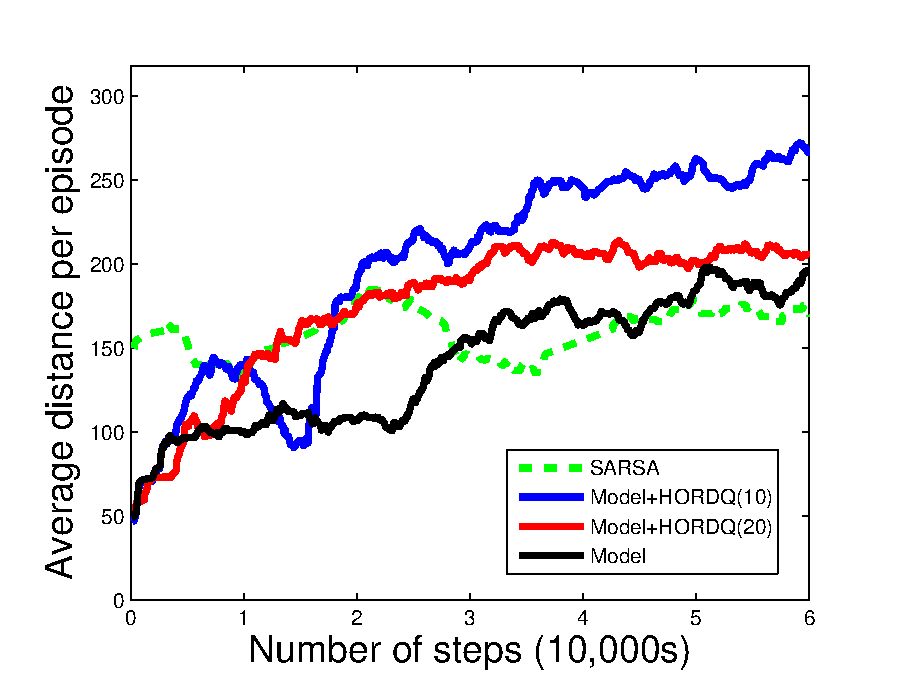
\includegraphics[width=4.0in] {./figures/1247.eps}
\end{center}
\end{minipage}

\caption{The distance that Mario moves for each episode, averaged over 20 episodes.
The parameters are $\alpha=0.05$ and $\gamma=0.7$. The exploration policy
$\epsilon$-greedy with $\epsilon = 0.01$.}
\label{fig:MarioExp}
\end{figure}


\begin{table}
    \begin{center}
\begin{tabular}[h]{l|l}
%\hline
%\multicolumn{1}{c}{}\\
\hline
Method Name & \# of finishing a level\\
\hline
SARSA    & 1\\
Model+HORDQ(10)    & 277\\
Model+HORDQ(20)     & 64\\
Model        & 0\\
\hline
\hline
\end{tabular}
\end{center}
\caption{The number of times for Mario to finish the level}
%\caption{The features used by predicates.}
\end{table}

%The exploration policy in model-free approach is enough to let Mario explore the 
%unknown actions. It is not necessary for model-based approach to have the exploration policy as well. 
%XX is a special hierarchy. It allows us to combine two different methods under the HRL
%framework even for a problem without clear hierarchical structure. 
%no overhead

The level is generated with Infinite Mario simulator of RL competition 2009. The random seed is 1247
with type 0 and the difficulty is 3.
The maximum distance for Mario to move to the right is 315.
Beyond that, the level is finished with +100 reward.

%Bruno when random seed 1247, are you talking about a specific run? If so, what's special about this one in specific? Is it typical of something?
%James No, it is not typical. It is just a random trial.

Table 1 shows the number of times for Mario to finish the level within 1000 episodes.
Unsurprisingly, the model-based and model-free method are difficult
to finish a level because they may fail to handle either monsters or pits.
The model-based method only includes the dynamics of Mario, and ignores the rest of effects in game.
Thus, the learned policy can get Mario killed. On the other hand, the features of model-free method
do not include the information of pits, so it may fall into a pit.

Figure \ref{fig:MarioExp} shows the distance travelled by Mario with different pseudo-rewards.
Unlike the experiment in the Bus domain, the model-based method does not have
a better learning rate then the model-free method. The problem is that the model-based method
may lead Mario to be killed by a monster in an early state, thus it suffers a decreased learning rate.

If we combine both methods, we can see that Mario now can learn a better policy since
it can avoid both pits and monsters.
If we increase the pseudo-reward, the chances for Mario to be killed will increase, as it follows
the action of model-based method more often.
If we decrease the pseudo-reward, the chances to fall into a pit will increase, as the model-free  
method ignores the pit completely.

Our approach actually suggests a way to mix different methods and learn a better policy.
\ \\
\ \\
\ \\
\ \\
\ \\
\ \\
\ \\
\ \\
\ \\
\ \\
\ \\
\ \\
\ \\
\ \\
\ \\
\ \\
\ \\
\ \\
\ \\
\ \\
\ \\
\ \\
\ \\
\ \\
\ \\
\ \\
\ \\
\ \\
\ \\
\ \\
\ \\
\ \\
\ \\
\ \\
\ \\
\ \\
\ \\
\ \\
\ \\
\ \\
\ \\
\ \\
\ \\
\ \\
\ \\
\ \\
\ \\
\ \\
\ \\
\ \\
\ \\
\ \\
\ \\
\ \\
\ \\
\ \\
\ \\
\ \\
\ \\
\ \\
\ \\
%From experiment, 
\endinput
%Most of the previous work on RL focus on model-free approaches for several reasons. 
%The most 
%Within a planning agent, there are at least two roles for real experience: it
%can be used to improve the model (to make it more accurately match the real
%environment) and it can be used to directly improve the value function and
%policy using the kinds of reinforcement learning methods we have discussed in
%previous chapters. The former we call model-learning, and the latter we call
%direct reinforcement learning (direct RL). The possible relationships between
%experience, model, values, and policy are summarized in Figure  9.2. Each arrow
%shows a relationship of influence and presumed improvement. Note how experience
%can improve value and policy functions either directly or indirectly via the
%model. It is the latter, which is sometimes called indirect reinforcement
%learning, that is involved in planning. 

%The second branch is model-based RL, which directly estimates
%a model of the environment and then plans with
%this model. Early work demonstrated that summarizing an
%agent’s experience into a model could be an efficient way
%to reuse data (Moore & Atkeson, 1993), and later work utilized
%the uncertainty in an agent’s model to guide exploration,
%yielding the first (probabilistic) finite bounds on the amount of data required
%to learn near-optimal behaviors in the general case (Kearns & Singh, 1998;
%Kakade, 2003).


%motivation: play a randomly generate maze to adapt to
%adapt to noval situation

%weakness-> an adversary to block the path forever
%no knowledge (coin won't disappear-->need hack to do it, moster won't move)
%comparison to the previous work->HRL,


%model based-> state space is too large. good to train with
%few examples (10 sec training)
%model free-> cannot handle randomly generated maze -> failed to adapt to noval situation. can handle large space (linear SARSA)
%Experiment: comparison with flat model based approach and hierarchical model based approach with approximation

%combine both-> use model based on top level to reduce
%the state space, and model free on bottom to 
%deal with randomized noisy world for short term reward

%build multilevel of hierachy on features
%label each room with a number 1, 2, 3
%the coordinate of wrt the room
%(1, (25, 30))
%move from room 1 to room 2
%top level
%action (1->2)
%second level
%assume (1, (25, 30)) -> (2, (0, 0))
%action ((25, 30) -> (0, 0)) goal (-25, -30) in single step

%need to build time model of the full state
%P(s->s'|x, t) the propability to move from state s to s'
%after t steps of the observation of full state x

%power coms from trasition model (model the shortest path), not shortest path
%you can use model-based approach on this

%fickle passenger of MaxQ
%coarseness on time and space scale

%-->you can work on continus varible now, no more grid world

%1. Assumption on the state difference (if it is not true --> like the agent in a world boundary or the health is 100 and cannot be imporve
  %since the state is outside the known state boundary, the planner whon't plan for it. but the local planner may still direct the agent
  %to go outside the world boundary, which may be a problem)
%2. Application to the hierachical RL
%3. Limitation: unachievable state (a coin surrounded by many monsters)
%4. Can inference in a very small world, not need to do 64 by 64
%Sometimes we need a plan. The greedy approach of reinforcement learning does not always work. 
%RL techniques have several limitations:
%1. It's difficult for to transfer the value function from a small world to a large one. If the agent has
%the experience only in a small world like 4 \times 4 grid, it cannot act well in 64 \times 64 grid
%because it does not know the correct action in regard to an object 63 grid away.

%2. It takes a long time to train the agent to be good enough. The greedy 

%3. The approximation only good in a small range. We need a plan for long term action.
%The noval state (the state in current game which has not been experienced) may 

%4. Impossible task to maze problems: RL require that optimal agent to find the optimal solution for a maze when all the features
%are input to the agent. Which is unlikely to work.(impractical when the maze is large)(unable to transfer
%the knowledge from previous maze experience to the current one) A practical solver shall invovle planning through 
%the possible route and find the one which can lead to the exist.
%All the work requires the agent to repeat play the same maze (assuming traps) until it finds the optimal solution.
%What if the maze changes every time?

%1. Is it guarranteed convergence? Yes, if we choose the goal next to the current state which leads to highest Q value. 
%It is the same as SARSA.
%2. How to choose the goal to guarrante convergence to optimal policy?

%Good to work on the problem with a long term reinforcement (feedback) like a maze.
%Bad to work with a problem with dynamic envirment (everything changes with or without agents actions)
%Bad when the consequence of an action is delayed for many steps. (poison)

%Q: prove that RL cannot solve maze problem
%Ability to transfer the knowledge from one maze to another
%compare the HRL in key-finding problem
%compare to the model-based RL





%application: the key-room problem--> each room lock a key, one room has a treasure, the agent needs to go through 
%a maze to collect the keys for each door and get the treasure

%Stochastic Shortest-Path Problems
%A Stochastic Shortest-Path problem is an mdp prob-
%lem in which the state space S = f1; : : : ; n; tg is such
%that t is a goal (target) state that is absorbing (i.e.,
%p(t; u; t) = 1 and g(t; u) = 0 for all u 2 U(t)), and the
%discount factor ® = 1. In this case, the existence of
%optimal policies (and optimal stationary policies) is a
%major mathematical problem. However, the existence
%is guarantee under the following reasonable conditions:
%(A1) There exists a policy that achieves the goal with
%probability 1 from any starting state.
%(A2) All costs are positive.
%The ¯rst assumption just expresses the fact that the
%problem admits a well-behaved solution. Such policies
%are known as proper policies. The second assumption,
%in the other hand, guarantees that all improper policies
%incurs in in¯nite cost for at least one state. Thus, both
%assumptions preclude cases where the optimal solution
%might \wander" around without never getting to the
%goal. For example, a problem having a zero-cost cycle
%(in state space) violates the second assumption.
%As mentioned in the Introduction, often we are only
%interested in knowing how to go from a ¯xed initial
%state, say 1, to the goal state. The optimal solution in
%this case is an partial optimal stationary policy ¹ such
%that ¹(i) = ¹¤(i) for all states i that are reachable
%from 1 when using the optimal policy ¹¤; the so-called
%relevant states when starting from 1.1
%Finding a partial optimal policy can be consider-
%ably simpler, the extreme case when the set of relevant
%states is ¯nite and the complete state space is in¯nite.
%Thus, the question of how to ¯nd partial optimal poli-
%cies is of great relevance. One algorithm for that is
%Real-Time Dynamic Programming.

%There are two ways for a RL agent to use its sample data. It can use the sample data to update the 
%value function and improve its policy. It is called model-free (or direct) reinforcement learning. 
%Another approach is to use the sample data to estimate parameters for the model of the environment and compute the value function
%from the model. It is called model-based (indirect) reinforcement learning.

%The advantage of model-based approaches is that they make more efficient use of the sample data, thus 
%it take fewer time to train a model-based RL agent. Other the other hand, model-free approaches do not assume 
%a prior model, so it would not be affected by the bias of the model design. Besides, the existence of 
%good linear approximation algorithms, such as linear SARSA, makes it possible for model-free approaches to
%handle large scale problems.

%Model-based approaches needs to enumerate through all possible states to compute the value function. 
%But the number of states grows exponentially with the number of features, 
%and it quickly becomes intractable if the number features grows large.

%The main idea of this work is to combine the model-free, model-based and hierarchical reinforcement learning.
%For the lower level of hierarchy, we adopt the model-free approach to handle the complete and possibly large state space.
%On the top level of hierarchy, we use the model-based to plan on a coarser level, which contains only small number of states.
%This approach allows the agent to plan on the higher level and make efficient use of the sample data. On the lower level,
%the agent uses model-free approaches with linear approximation to handle the complete state space.

%The prior works on hierarchical reinforcement learning (HRL) can be divided into two categories: model-free and model-based approaches. 
%The model-free approaches include HAMQ \cite{HAMQ}, MAXQ \cite{MAXQ}, SMDP and options framework \cite{option}
%For model-based approaches, Seri et al. \cite{HLearning} proposed a model-based HRL in average reward setting.
%Diuk et al. \cite{Diuk} adopted model-based HRL to deterministic domain. Jong and Stone \cite{RMaxQ} combined 
%R-MAXQ and MAXQ to achieve efficient model-based exploration and the action abstraction of MAXQ.

%TODO: show that model based state difference can learn randomly generated maze with very limited steps (only four touches of the wall)
%TODO: use a poison example to show the limit of pure approximated model-based approach and the motivation
%of use hierarchical optimal policy for pseudo reward and recursive optimal policy for real reward. It can be shown that
%it will converge to optimal policy if the true goal state of the game is included as a subgoal(
%the worst case is the child node finish the game by itself)

\chapter{Conclusions}

%Our result suggests the possibility incorporating a wide range of planning
%techniques such as STRIPS [11] or object-oriented RL [16] into the HRL framework without the
%loss of optimality. One future direction is to investigate the applicability of combining our method
%with such techniques.

Model-based methods are powerful tools. It allows us to predict the outcome 
of the agent behavior and plan over it. They can effectively reduce the number of 
samples which are required to find the optimal policy.
However, model-based methods may not be able to learn the optimal
policy due to the structural assumptions.
%However, model-based methods may not be able to learn the transition function correctly.
%The possible reasons are:
%\begin{itemize}
%\item The inaccuracy in the supervised learning algorithms
%\item The numerical imprecision in the continuous case
%\item It is not possible to learn all the effects
%\item It would be time-consuming if we compute all possible effects during planning process
%\end{itemize}
In this work, we propose an approach to combine the approximate model-based method with the
model-free method (HORDQ) under the HRL framework. We are able to show that our approach
can learn the optimal policy even when the assumption of model is not satisfied. Furthermore, we show that the optimality
is guaranteed for any subtask policy as long as the subtask does not belong to the total leaf
cover of given hierarchy.

In this chapter, we share our experience about how to apply our theory to design a system.
Since the performance of system highly depends on the value of pseudo-reward, we will also introduce
some heuristics for choosing an appropriate pseudo-reward.
Finally, we discuss the limitation and possible future works of our theory. 

%In this thesis, we describe an approach to use model-free methods to 
%compensate the scenarios when model-based methods are failed to learn the optimal policy.
%In small problems which we can use table-lookup methods, it is guaranteed to learn the optimal
%policy. 
%For large problems, there are no guarantee, but we should 
%The choice of features of model-free methods effect the overall performance
%If we put too much irrelevant features, the qualify of learned policy will be severed.

\section{System design}

An important design principle of the system is to design the model-based method first,
and the model-free method later. 
We need to decide the features used by the
model-based methods, the underlying supervised learning algorithms and most
importantly, the effects which we would like to include in our model. Then we
run the experiments, and observe the scenarios where the model-based method
is failed. 
Based on the observations, we design a set of features for model-free methods to handle
these scenarios. Note that we don't need to design a set of features to handle
the whole problems, but only part of it. We only need the model-free method
to take control when the model-based method fails. Therefore, we can reduce the
number of features for model-free methods and let the overall system
successfully handle all scenarios.

%//There are other alternative approaches to overcome their limitation.
Since our work is about how to use model-free methods to improve the learned policy of model-based methods,
it is not necessary to adopt our work if model-based methods can learn the optimal policy
on their own.

Our work is not the only solution when model-based methods fail.
Another alternative is to improve the quality of the model by including more domain knowledge.
For example, in our Infinite Mario experiment, we do not include any effects 
of the interactions between monsters and Mario. It is possible to
hand-code the preconditions and postconditions of these effects, as Walsh et al. proposed in \cite{Walsh09}.
In fact, the source code of Infinite Mario is publicly available.
%(TODO: source code)
There are no need to use model-based methods to learn the model. Instead,
we can simulate the experiences of the agent with the simulator of Infinite Mario. 
Since the environment and the model are identical, there are no biases which will be 
introduced during the simulation process.
It is what Baumgarten did with his $A^*$ method for Mario AI\cite{Robin09}.
With the complete domain knowledge, it is unlikely for any RL methods to outperform his work.

However, the key idea of RL is to build an adaptive agent.
Not only do we want the agent to perform well in a problem which we know very well,
but we also want the agent to adapt itself to novel problems which we cannot foresee when we design the agent.
If we put too much domain knowledge into the agent's design, we forbids it from adapting 
itself when the prior knowledge does not hold anymore. 
In this work, we introduce an alternative -- instead of designing an omnipotent model-based agent, we
divide the learning task into different parts and let model-free methods handle the parts which model-based methods cannot do.

%We want the agent to adapt itself to novel scenarios and find the optimal policy.
%If we put too much domain knowledge into the design of the model, the agent 
%will not be able to adapt when the knowledge does not hold in these scenarios.
%If we put too less, the model may be poor-approximated, 
%and hinder the learning process. 
%(TODO: my school bus exp)
%Our work tries to find a balance between 


%TODO: relationship with HRL (no 
%Although we use HRL framework to incorporate model-based and model-free methods, 
%TODO: the choice of model-free methods (not only HORDQ), anything that can know its consquences  
%It is not a problem to find a hierarchy

\section{Choose an appropriate pseudo-reward}
It is important to choose an appropriate pseudo-reward. If we choose a pseudo-reward which is too small, 
the policy of the agent will be similar to the policy of model-free method. Therefore, we may lose the 
benefit of faster learning rate. On the other hand, if the pseudo-reward is too large, 
the policy will be similar to the model-model method, which may be suboptimal
when the assumptions of the model are not all satisfied.

It is easy to determine when a pseudo-reward is too large by
looking at the difference between the expected reward of the optimal policy and the policy of model-based method.
If a pseudo-reward is larger than the difference, the model-free method will follow the policy
of the model-based method strictly, and the combined policy will be the same as 
the policy of model-based method.

In our experiments (Sections \ref{se:BusRes} and \ref{se:MarioRes}), a pseudo-reward larger than the expected death penalty is considered "too large", 
since it will let the model-free method follow the instruction of model-based method even 
when it will result in the death of the agent. If we choose a pseudo-reward which is smaller than it,
the model-free method will choose an action that avoids the death of the agent.

It is more difficult to decide if the pseudo-reward is large enough. 
For small problems, if we adopt table-lookup HORDQ as the model-free method,
the optimal policy will be learned when the pseudo-reward is decreased to zero.
So a viable strategy is to choose some pseudo-reward, which is not too large, and
gradually decrease it to zero.
For large problems, we have adopt model-free methods with function approximation techniques
, therefore the optimal policy might not be learned when the pseudo-reward is zero.
Instead, we need to find out an optimal pseudo-reward which can maximize the expected reward.
A way to decide it is to conduct the experiment with the model-free method,
and choose a pseudo-reward which is large enough to encourage
the model-free method to follow the policy of model-based one.
%It is necessary to have a large pseudo-reward in the beginning since 
%the model-based method does not have enough samples to build a good model,
%it is possible for it to compute very poor policy.

\section{Limitation and future work}

The quality of learned policy depends on the chosen model-free method,
the model-based method and the pseudo-reward. 
Since we can control the pseudo-reward to decide if the combined
policy should be similar to model-free or model-based one,
the combined policy can never be worse than any of them. 

Since our work is a combination of two,  Our work will fail in scenarios where both methods fail, 
It is only possible to resolve it by applying better model-free or model-based methods. 

%If we adopt the task hierarchy in \ref{se:MarioExp}, we can apply our work
%to any reinforcement learning problems.  
%The limitation of the applicability
%of our work actually comes from the underlying RL methods. 

Nevertheless, our work is not be useful when one method outperforms another.
In general, model-based methods learn faster than model-free methods because of
efficient use of samples, but it may not be true for some problems. 
If the chosen model-based method is worse than the model-free method in both learning
rate and the learned policy, it is pointless to combine both methods. 
Similarly, if the model-free method fails to handle the scenarios where the model-based
method fails or the model-based method can learn the optimal policy, it is not necessary to apply our work.
For small problems, if the model-based method fails to learn the optimal policy, 
we learn the optimal policy by combining it with table-lookup HORDQ as we prove in Theorem \ref{thm:opt}.
For large problems, it is difficult since approximated model-free RL may not learn the optimal policy.
It is necessary to have the knowledge about the domain and apply the knowledge to choose some good features.

%TODO: the process is similar to model-free RL
We introduced the theory of improving the quality of the policy of model-based methods. However, we don't have any theory regarding the learning rate.
It is true that if the model-based method is "approximately good", we can enjoy the 
faster learning rate, as we showed in the experiment of Bus domain. Nevertheless, there are no theory
to tell if a model-based method is approximately good or not.
A possible direction of future work is to investigate what kind of the properties of model-based
methods are necessary to increase the learning rate and how much they can increase when they are combined with model-free methods.




%1. No theory about learning rate (what is a good approximation?)
%2. No thery about the interaction betwwen model-based and model-free approach.
%If model-base dapproahc does not change it's policy accroding to model-free's policy,
%the learning can be slower than pure model-free. Since model-based method
%will stick on it's original bad plan, and guid the agent to the wrong action.

%A problem may arise when the pseudo-reward is 

%The performance of our approach depends on 
%Large enough so that the model-free approach will pursue the subgoal
%When the model-based approach doesn’t have enough samples to build an approximately good model
%Small enough to pass the control to model-free approach when the model-based approach doesn’t work

%Combine both model-free and model-based approaches
%Overcome the structure assumption of model-based approaches
%Learns a better policy by mixing these approaches
%Designing pseudo-reward requires insight of the problem
%No theory yet!

%model-based or model-free is too good

%We have presented a learning algorithm for agile, integrated whole-body
%skills of physically-simulated characters. The algorithm uses a nature-inspired
%online, active exploration of the character action space to nd reliable mo-
%tions that give rise to parameterized skills. We further demonstrated that
%our algorithm works for a family of simple characters without requiring any
%algorithm or parameter modications. In addition, we experimented with
%a complex dog character in 3-D and showed that our approach generalizes
%to this character, given appropriate changes in the motor abstractions used
%during the learning process. Finally, we showed that the resulting parame-
%a terrain.
%5.1 Discussion
%While a learning approach to acquiring skills possesses many benets, it also
%comes with its own set of limitations.
%Mainly, we found that the learning process requires occasional super-
%vision to ensure that the intended skills are actually being learned. For
%example in one case, a character learned a Flip motion that made it launch
%necessary to supervise the learning process and restart it on a few occasions.
%The majority of skill and character combinations (roughly 90%) did not re-
%quire any interventions. We believe that these issues could be alleviated by
%better quantifying when a particular trial should count as being successful

%for every skill.
%In addition, the phase 1 reward functions may be dicult to specify in
%some cases. In particular, we found the GetUp skill to be the most trou-
%blesome. If the character fails at getting up after some Motor Action, how
%should one assign a score for how close the attempt was? Specifying a bad
%phase 1 reward function could lead to long computation times in phase 1,
%because the character is essentially left searching randomly in the motor
%space for a successful action. Even worse, the optimization in phase 1 could
%be repeatedly led astray with an inappropriately specied phase 1 reward
%function.
%The main challenges for the quadruped character were aesthetic in na-
%ture. Unlike the Acrobot's motions, a dog's leap is a specic type of motion
%that we are all familiar with from nature. Even though the learning al-
%gorithm produced leaps that accomplished all desired goals, they did not
%always resemble leaps that one would expect to see from a real dog. For
%but this motion did not emerge in the actions that were produced by the
%algorithm. Instead, the dog left its front feet outstretched during the leap,
%producing a motion that felt qualitatively strange despite achieving all task
%goals. In the end, we opted to include these details into the leap controller
%manually to achieve a more familiar style of motion.
%5.2 Limitations and future work
%Even though the learning algorithm described in this thesis works well for
%our characters and the set of skills we considered, we make no claims to
%have addressed the general problem of motor learning. In this section, we
%discuss possible extensions of the proposed framework that can bring us
%closer toward the nal goal of matching human or animal abilities.
%To begin with, several immediate improvements can be made to the
%framework by addressing some of the simplications that were made mostly


%\include{conclusions}

%    3. Notes
%    4. Footnotes

%    5. Bibliography
\begin{singlespace}
\raggedright
\bibliographystyle{abbrvnat}
\bibliography{biblio}
\end{singlespace}

\appendix
%    6. Appendices (including copies of all required UBC Research
%       Ethics Board's Certificates of Approval)
%\include{reb-coa}	% pdfpages is useful here

\backmatter
%    7. Index
% See the makeindex package: the following page provides a quick overview
% <http://www.image.ufl.edu/help/latex/latex_indexes.shtml>


\end{document}
